\appendix


%% CONTINUE: Monochromatic cow theorem.
%% CONTINUE: 1 = 2.
%% CONTINUE: Buchner Coefficients.
%% CONTINUE: Mauch's theorem.
%% CONTINUE: Unit conversions to beers.

%% CONTINUE: Infinite space Green functions
%% CONTINUE: Green functions for partial differential equations.
%% CONTINUE: update the chapter in definite integrals

%%
%% Add the picture in the complex variables section.
%%
%% Beef up the linear algebra section with some material on matrices.
%% Make sure to have all the background necessary for the Wronskian and tolo.
%%
%% Add the integral of $x \sin x$ etc.
%%
%% Add Bessel functions to the table of Taylor series.
%%
%% Add hyperbolic identities to the trig section.
%%
%% Are the range restrictions in the table of derivatives necessary?
%%
%% Verify the table of derivatives
%%
%% Add a table of differential equations.
%%



%%===========================================================================
%%===========================================================================
\chapter{GNU Free Documentation License}
\label{label_fdl}

 \begin{center}

       Version 1.2, November 2002


 Copyright \copyright 2000,2001,2002  Free Software Foundation, Inc.
 
 \bigskip
 
     51 Franklin St, Fifth Floor, Boston, MA  02110-1301  USA
  
 \bigskip
 
 Everyone is permitted to copy and distribute verbatim copies
 of this license document, but changing it is not allowed.
\end{center}


\begin{center}
{\bf\large Preamble}
\end{center}

The purpose of this License is to make a manual, textbook, or other
functional and useful document "free" in the sense of freedom: to
assure everyone the effective freedom to copy and redistribute it,
with or without modifying it, either commercially or noncommercially.
Secondarily, this License preserves for the author and publisher a way
to get credit for their work, while not being considered responsible
for modifications made by others.

This License is a kind of "copyleft", which means that derivative
works of the document must themselves be free in the same sense.  It
complements the GNU General Public License, which is a copyleft
license designed for free software.

We have designed this License in order to use it for manuals for free
software, because free software needs free documentation: a free
program should come with manuals providing the same freedoms that the
software does.  But this License is not limited to software manuals;
it can be used for any textual work, regardless of subject matter or
whether it is published as a printed book.  We recommend this License
principally for works whose purpose is instruction or reference.


\begin{center}
{\Large\bf 1. APPLICABILITY AND DEFINITIONS}
\addcontentsline{toc}{section}{1. APPLICABILITY AND DEFINITIONS}
\end{center}

This License applies to any manual or other work, in any medium, that
contains a notice placed by the copyright holder saying it can be
distributed under the terms of this License.  Such a notice grants a
world-wide, royalty-free license, unlimited in duration, to use that
work under the conditions stated herein.  The \textbf{"Document"}, below,
refers to any such manual or work.  Any member of the public is a
licensee, and is addressed as \textbf{"you"}.  You accept the license if you
copy, modify or distribute the work in a way requiring permission
under copyright law.

A \textbf{"Modified Version"} of the Document means any work containing the
Document or a portion of it, either copied verbatim, or with
modifications and/or translated into another language.

A \textbf{"Secondary Section"} is a named appendix or a front-matter section of
the Document that deals exclusively with the relationship of the
publishers or authors of the Document to the Document's overall subject
(or to related matters) and contains nothing that could fall directly
within that overall subject.  (Thus, if the Document is in part a
textbook of mathematics, a Secondary Section may not explain any
mathematics.)  The relationship could be a matter of historical
connection with the subject or with related matters, or of legal,
commercial, philosophical, ethical or political position regarding
them.

The \textbf{"Invariant Sections"} are certain Secondary Sections whose titles
are designated, as being those of Invariant Sections, in the notice
that says that the Document is released under this License.  If a
section does not fit the above definition of Secondary then it is not
allowed to be designated as Invariant.  The Document may contain zero
Invariant Sections.  If the Document does not identify any Invariant
Sections then there are none.

The \textbf{"Cover Texts"} are certain short passages of text that are listed,
as Front-Cover Texts or Back-Cover Texts, in the notice that says that
the Document is released under this License.  A Front-Cover Text may
be at most 5 words, and a Back-Cover Text may be at most 25 words.

A \textbf{"Transparent"} copy of the Document means a machine-readable copy,
represented in a format whose specification is available to the
general public, that is suitable for revising the document
straightforwardly with generic text editors or (for images composed of
pixels) generic paint programs or (for drawings) some widely available
drawing editor, and that is suitable for input to text formatters or
for automatic translation to a variety of formats suitable for input
to text formatters.  A copy made in an otherwise Transparent file
format whose markup, or absence of markup, has been arranged to thwart
or discourage subsequent modification by readers is not Transparent.
An image format is not Transparent if used for any substantial amount
of text.  A copy that is not "Transparent" is called \textbf{"Opaque"}.

Examples of suitable formats for Transparent copies include plain
ASCII without markup, Texinfo input format, LaTeX input format, SGML
or XML using a publicly available DTD, and standard-conforming simple
HTML, PostScript or PDF designed for human modification.  Examples of
transparent image formats include PNG, XCF and JPG.  Opaque formats
include proprietary formats that can be read and edited only by
proprietary word processors, SGML or XML for which the DTD and/or
processing tools are not generally available, and the
machine-generated HTML, PostScript or PDF produced by some word
processors for output purposes only.

The \textbf{"Title Page"} means, for a printed book, the title page itself,
plus such following pages as are needed to hold, legibly, the material
this License requires to appear in the title page.  For works in
formats which do not have any title page as such, "Title Page" means
the text near the most prominent appearance of the work's title,
preceding the beginning of the body of the text.

A section \textbf{"Entitled XYZ"} means a named subunit of the Document whose
title either is precisely XYZ or contains XYZ in parentheses following
text that translates XYZ in another language.  (Here XYZ stands for a
specific section name mentioned below, such as \textbf{"Acknowledgements"},
\textbf{"Dedications"}, \textbf{"Endorsements"}, or \textbf{"History"}.)  
To \textbf{"Preserve the Title"}
of such a section when you modify the Document means that it remains a
section "Entitled XYZ" according to this definition.

The Document may include Warranty Disclaimers next to the notice which
states that this License applies to the Document.  These Warranty
Disclaimers are considered to be included by reference in this
License, but only as regards disclaiming warranties: any other
implication that these Warranty Disclaimers may have is void and has
no effect on the meaning of this License.


\begin{center}
{\Large\bf 2. VERBATIM COPYING}
\addcontentsline{toc}{section}{2. VERBATIM COPYING}
\end{center}

You may copy and distribute the Document in any medium, either
commercially or noncommercially, provided that this License, the
copyright notices, and the license notice saying this License applies
to the Document are reproduced in all copies, and that you add no other
conditions whatsoever to those of this License.  You may not use
technical measures to obstruct or control the reading or further
copying of the copies you make or distribute.  However, you may accept
compensation in exchange for copies.  If you distribute a large enough
number of copies you must also follow the conditions in section 3.

You may also lend copies, under the same conditions stated above, and
you may publicly display copies.


\begin{center}
{\Large\bf 3. COPYING IN QUANTITY}
\addcontentsline{toc}{section}{3. COPYING IN QUANTITY}
\end{center}


If you publish printed copies (or copies in media that commonly have
printed covers) of the Document, numbering more than 100, and the
Document's license notice requires Cover Texts, you must enclose the
copies in covers that carry, clearly and legibly, all these Cover
Texts: Front-Cover Texts on the front cover, and Back-Cover Texts on
the back cover.  Both covers must also clearly and legibly identify
you as the publisher of these copies.  The front cover must present
the full title with all words of the title equally prominent and
visible.  You may add other material on the covers in addition.
Copying with changes limited to the covers, as long as they preserve
the title of the Document and satisfy these conditions, can be treated
as verbatim copying in other respects.

If the required texts for either cover are too voluminous to fit
legibly, you should put the first ones listed (as many as fit
reasonably) on the actual cover, and continue the rest onto adjacent
pages.

If you publish or distribute Opaque copies of the Document numbering
more than 100, you must either include a machine-readable Transparent
copy along with each Opaque copy, or state in or with each Opaque copy
a computer-network location from which the general network-using
public has access to download using public-standard network protocols
a complete Transparent copy of the Document, free of added material.
If you use the latter option, you must take reasonably prudent steps,
when you begin distribution of Opaque copies in quantity, to ensure
that this Transparent copy will remain thus accessible at the stated
location until at least one year after the last time you distribute an
Opaque copy (directly or through your agents or retailers) of that
edition to the public.

It is requested, but not required, that you contact the authors of the
Document well before redistributing any large number of copies, to give
them a chance to provide you with an updated version of the Document.


\begin{center}
{\Large\bf 4. MODIFICATIONS}
\addcontentsline{toc}{section}{4. MODIFICATIONS}
\end{center}

You may copy and distribute a Modified Version of the Document under
the conditions of sections 2 and 3 above, provided that you release
the Modified Version under precisely this License, with the Modified
Version filling the role of the Document, thus licensing distribution
and modification of the Modified Version to whoever possesses a copy
of it.  In addition, you must do these things in the Modified Version:

\begin{itemize}
\item[A.] 
   Use in the Title Page (and on the covers, if any) a title distinct
   from that of the Document, and from those of previous versions
   (which should, if there were any, be listed in the History section
   of the Document).  You may use the same title as a previous version
   if the original publisher of that version gives permission.
   
\item[B.]
   List on the Title Page, as authors, one or more persons or entities
   responsible for authorship of the modifications in the Modified
   Version, together with at least five of the principal authors of the
   Document (all of its principal authors, if it has fewer than five),
   unless they release you from this requirement.
   
\item[C.]
   State on the Title page the name of the publisher of the
   Modified Version, as the publisher.
   
\item[D.]
   Preserve all the copyright notices of the Document.
   
\item[E.]
   Add an appropriate copyright notice for your modifications
   adjacent to the other copyright notices.
   
\item[F.]
   Include, immediately after the copyright notices, a license notice
   giving the public permission to use the Modified Version under the
   terms of this License, in the form shown in the Addendum below.
   
\item[G.]
   Preserve in that license notice the full lists of Invariant Sections
   and required Cover Texts given in the Document's license notice.
   
\item[H.]
   Include an unaltered copy of this License.
   
\item[I.]
   Preserve the section Entitled "History", Preserve its Title, and add
   to it an item stating at least the title, year, new authors, and
   publisher of the Modified Version as given on the Title Page.  If
   there is no section Entitled "History" in the Document, create one
   stating the title, year, authors, and publisher of the Document as
   given on its Title Page, then add an item describing the Modified
   Version as stated in the previous sentence.
   
\item[J.]
   Preserve the network location, if any, given in the Document for
   public access to a Transparent copy of the Document, and likewise
   the network locations given in the Document for previous versions
   it was based on.  These may be placed in the "History" section.
   You may omit a network location for a work that was published at
   least four years before the Document itself, or if the original
   publisher of the version it refers to gives permission.
   
\item[K.]
   For any section Entitled "Acknowledgements" or "Dedications",
   Preserve the Title of the section, and preserve in the section all
   the substance and tone of each of the contributor acknowledgements
   and/or dedications given therein.
   
\item[L.]
   Preserve all the Invariant Sections of the Document,
   unaltered in their text and in their titles.  Section numbers
   or the equivalent are not considered part of the section titles.
   
\item[M.]
   Delete any section Entitled "Endorsements".  Such a section
   may not be included in the Modified Version.
   
\item[N.]
   Do not retitle any existing section to be Entitled "Endorsements"
   or to conflict in title with any Invariant Section.
   
\item[O.]
   Preserve any Warranty Disclaimers.
\end{itemize}

If the Modified Version includes new front-matter sections or
appendices that qualify as Secondary Sections and contain no material
copied from the Document, you may at your option designate some or all
of these sections as invariant.  To do this, add their titles to the
list of Invariant Sections in the Modified Version's license notice.
These titles must be distinct from any other section titles.

You may add a section Entitled "Endorsements", provided it contains
nothing but endorsements of your Modified Version by various
parties--for example, statements of peer review or that the text has
been approved by an organization as the authoritative definition of a
standard.

You may add a passage of up to five words as a Front-Cover Text, and a
passage of up to 25 words as a Back-Cover Text, to the end of the list
of Cover Texts in the Modified Version.  Only one passage of
Front-Cover Text and one of Back-Cover Text may be added by (or
through arrangements made by) any one entity.  If the Document already
includes a cover text for the same cover, previously added by you or
by arrangement made by the same entity you are acting on behalf of,
you may not add another; but you may replace the old one, on explicit
permission from the previous publisher that added the old one.

The author(s) and publisher(s) of the Document do not by this License
give permission to use their names for publicity for or to assert or
imply endorsement of any Modified Version.


\begin{center}
{\Large\bf 5. COMBINING DOCUMENTS}
\addcontentsline{toc}{section}{5. COMBINING DOCUMENTS}
\end{center}


You may combine the Document with other documents released under this
License, under the terms defined in section 4 above for modified
versions, provided that you include in the combination all of the
Invariant Sections of all of the original documents, unmodified, and
list them all as Invariant Sections of your combined work in its
license notice, and that you preserve all their Warranty Disclaimers.

The combined work need only contain one copy of this License, and
multiple identical Invariant Sections may be replaced with a single
copy.  If there are multiple Invariant Sections with the same name but
different contents, make the title of each such section unique by
adding at the end of it, in parentheses, the name of the original
author or publisher of that section if known, or else a unique number.
Make the same adjustment to the section titles in the list of
Invariant Sections in the license notice of the combined work.

In the combination, you must combine any sections Entitled "History"
in the various original documents, forming one section Entitled
"History"; likewise combine any sections Entitled "Acknowledgements",
and any sections Entitled "Dedications".  You must delete all sections
Entitled "Endorsements".

\begin{center}
{\Large\bf 6. COLLECTIONS OF DOCUMENTS}
\addcontentsline{toc}{section}{6. COLLECTIONS OF DOCUMENTS}
\end{center}

You may make a collection consisting of the Document and other documents
released under this License, and replace the individual copies of this
License in the various documents with a single copy that is included in
the collection, provided that you follow the rules of this License for
verbatim copying of each of the documents in all other respects.

You may extract a single document from such a collection, and distribute
it individually under this License, provided you insert a copy of this
License into the extracted document, and follow this License in all
other respects regarding verbatim copying of that document.


\begin{center}
{\Large\bf 7. AGGREGATION WITH INDEPENDENT WORKS}
\addcontentsline{toc}{section}{7. AGGREGATION WITH INDEPENDENT WORKS}
\end{center}


A compilation of the Document or its derivatives with other separate
and independent documents or works, in or on a volume of a storage or
distribution medium, is called an "aggregate" if the copyright
resulting from the compilation is not used to limit the legal rights
of the compilation's users beyond what the individual works permit.
When the Document is included in an aggregate, this License does not
apply to the other works in the aggregate which are not themselves
derivative works of the Document.

If the Cover Text requirement of section 3 is applicable to these
copies of the Document, then if the Document is less than one half of
the entire aggregate, the Document's Cover Texts may be placed on
covers that bracket the Document within the aggregate, or the
electronic equivalent of covers if the Document is in electronic form.
Otherwise they must appear on printed covers that bracket the whole
aggregate.


\begin{center}
{\Large\bf 8. TRANSLATION}
\addcontentsline{toc}{section}{8. TRANSLATION}
\end{center}


Translation is considered a kind of modification, so you may
distribute translations of the Document under the terms of section 4.
Replacing Invariant Sections with translations requires special
permission from their copyright holders, but you may include
translations of some or all Invariant Sections in addition to the
original versions of these Invariant Sections.  You may include a
translation of this License, and all the license notices in the
Document, and any Warranty Disclaimers, provided that you also include
the original English version of this License and the original versions
of those notices and disclaimers.  In case of a disagreement between
the translation and the original version of this License or a notice
or disclaimer, the original version will prevail.

If a section in the Document is Entitled "Acknowledgements",
"Dedications", or "History", the requirement (section 4) to Preserve
its Title (section 1) will typically require changing the actual
title.


\begin{center}
{\Large\bf 9. TERMINATION}
\addcontentsline{toc}{section}{9. TERMINATION}
\end{center}


You may not copy, modify, sublicense, or distribute the Document except
as expressly provided for under this License.  Any other attempt to
copy, modify, sublicense or distribute the Document is void, and will
automatically terminate your rights under this License.  However,
parties who have received copies, or rights, from you under this
License will not have their licenses terminated so long as such
parties remain in full compliance.


\begin{center}
{\Large\bf 10. FUTURE REVISIONS OF THIS LICENSE}
\addcontentsline{toc}{section}{10. FUTURE REVISIONS OF THIS LICENSE}
\end{center}


The Free Software Foundation may publish new, revised versions
of the GNU Free Documentation License from time to time.  Such new
versions will be similar in spirit to the present version, but may
differ in detail to address new problems or concerns.  See
http://www.gnu.org/copyleft/.

Each version of the License is given a distinguishing version number.
If the Document specifies that a particular numbered version of this
License "or any later version" applies to it, you have the option of
following the terms and conditions either of that specified version or
of any later version that has been published (not as a draft) by the
Free Software Foundation.  If the Document does not specify a version
number of this License, you may choose any version ever published (not
as a draft) by the Free Software Foundation.



















%%===========================================================================
%%===========================================================================
\chapter{Greek Letters}
\raggedbottom 

\paragraph{}
The following table shows the greek letters, (some of them have two 
typeset variants), and their corresponding Roman letters.

\setlongtables
\begin{longtable}{l|lll}
  \emph{Name} & \emph{Roman} & \emph{Lower} & \emph{Upper} \\
  \hline
  alpha & a & $\alpha$ & \\
  beta & b & $\beta$ & \\
  chi & c & $\chi$ & \\
  delta & d & $\delta$ & $\Delta$ \\
  epsilon & e & $\epsilon$ & \\
  epsilon (variant) & e & $\varepsilon$ & \\
  phi & f & $\phi$ & $\Phi$ \\
  phi (variant) & f & $\varphi$ & \\
  gamma & g & $\gamma$ & $\Gamma$ \\
  eta & h & $\eta$ & \\
  iota & i & $\iota$ & \\
  kappa & k & $\kappa$ & \\
  lambda & l & $\lambda$ & $\Lambda$ \\
  mu & m & $\mu$ & \\
  nu & n & $\nu$ & \\
  omicron & o & $o$ & \\
  pi & p & $\pi$ & $\Pi$ \\
  pi (variant) & p & $\varpi$ & \\
  theta & q & $\theta$ & $\Theta$ \\
  theta (variant) & q & $\vartheta$ & \\
  rho & r & $\rho$ & \\
  rho (variant) & r & $\varrho$ & \\
  sigma & s & $\sigma$ & $\Sigma$ \\
  sigma (variant) & s & $\varsigma$ & \\
  tau & t & $\tau$ & \\
  upsilon & u & $\upsilon$ & $\Upsilon$ \\
  omega & w & $\omega$ & $\Omega$ \\
  xi & x & $\xi$ & $\Xi$ \\
  psi & y & $\psi$ & $\Psi$ \\
  zeta & z & $\zeta$ & 
\end{longtable}















\raggedbottom
%%===========================================================================
%%===========================================================================
\chapter{Notation}
\raggedbottom 


%% CONTINUE: add special functions, like Airy, Legendre,...

\setlongtables
\begin{longtable}{ll}
  $C$             & class of continuous functions \\
  $C^n$           & class of $n$-times continuously differentiable functions \\
  $\mathbb{C}$    & set of complex numbers \\
  $\delta(x)$ & Dirac delta function \\
  $\mathcal{F}[\cdot]$       & Fourier transform \\
  $\mathcal{F}_c[\cdot]$     & Fourier cosine transform \\
  $\mathcal{F}_s[\cdot]$     & Fourier sine transform \\
  $\gamma$            & Euler's constant, 
  $\gamma = \int_0^\infty e^{-x} \Log x \,d x$ \\
  $\Gamma(\nu)$        & Gamma function \\
  $H(x)$          & Heaviside function \\
  $H_\nu^{(1)}(x)$ & Hankel function of the first kind and order $\nu$ \\
  $H_\nu^{(2)}(x)$ & Hankel function of the second kind and order $\nu$ \\
  $\imath$ & $\imath \equiv \sqrt{-1}$ \\
  $J_\nu(x)$       & Bessel function of the first kind and order $\nu$ \\
  $K_\nu(x)$       & Modified Bessel function of the first kind and order $\nu$ \\
  $\mathcal{L}[\cdot]$       & Laplace transform \\
  $\mathbb{N}$    & set of natural numbers, (positive integers) \\
  $N_\nu(x)$       & Modified Bessel function of the second kind and order $\nu$\\
  $\mathbb{R}$    & set of real numbers \\
  $\mathbb{R}^+$  & set of positive real numbers \\
  $\mathbb{R}^-$  & set of negative real numbers \\
  $o(z)$          & terms smaller than $z$ \\
  $\mathcal{O}(z)$        & terms no bigger than $z$ \\
  $\textpv\int$     & principal value of the integral \\
  $\psi(\nu)$        & digamma function, 
  $\psi(\nu) = \frac{\dd}{\dd \nu} \log \Gamma(\nu)$ \\
  $\psi^{(n)}(\nu)$  & polygamma function, 
  $\psi^{(n)}(\nu) = \frac{d^n}{d \nu^n} \psi(\nu)$ \\
  $u^{(n)}(x)$    & $\frac{\partial^n u}{\partial x^n}$ \\
  $u^{(n,m)}(x,y)$        & $\frac{\partial^{n+m}u}{\partial x^n \partial y^m}$ \\
  $Y_\nu(x)$       & Bessel function of the second kind and order $\nu$,
  Neumann function \\
  $\mathbb{Z}$    & set of integers \\
  $\mathbb{Z}^+$  & set of positive integers 
\end{longtable}





%%%% CONTINUE
%%%% define the ---jectives




\raggedbottom
%%=============================================================================
%%=============================================================================
\chapter{Formulas from Complex Variables}
\flushbottom


\paragraph{Analytic Functions.}
\index{analytic functions}
A function $f(z)$ is analytic in a domain if the derivative $f'(z)$ 
exists in that domain.

If $f(z) = u(x, y) + \imath v(x, y)$ is defined in some neighborhood of
$z_0 = x_0 + \imath y_0$ and the partial derivatives of $u$ and $v$ are
continuous and satisfy the \textbf{Cauchy-Riemann equations}
\index{Cauchy-Riemann equations}
\[
u_x = v_y, \qquad u_y = - v_x,
\]
then $f'(z_0)$ exists.

\paragraph{Residues.}
\index{residues}
\index{Laurent expansions}
If $f(z)$ has the Laurent expansion
\[ 
f(z) = \sum_{n=-\infty}^{\infty} a_n z^n, 
\]
then the residue of $f(z)$ at $z = z_0$ is
\[ 
\Res(f(z),z_0) = a_{-1}.
\]



\paragraph{Residue Theorem.}
\index{residue theorem}
Let $C$ be a positively oriented, simple, closed contour.  If $f(z)$ is
analytic in and on $C$ except for isolated singularities at $z_1, z_2, \ldots,
z_N$ inside $C$ then
\[ 
\oint_C f(z)\,dz = \imath 2 \pi \sum_{n=1}^N \Res(f(z),z_n).
\]
If in addition $f(z)$ is analytic outside $C$ in the finite complex plane
then
\[ 
\oint_C f(z)\,dz = \imath 2 \pi \Res\left( \frac{1}{z^2} f\left( \frac{1}{z} \right),
  0\right).
\]



\paragraph{Residues of a pole of order $\mathbf{n}$.}
\index{residues!of a pole of order $n$}
If $f(z)$ has a pole of order $n$ at $z=z_0$ then 
\[ 
\Res(f(z),z_0) = \lim_{z \to z_0} \left( \frac{1}{(n-1)!} 
  \frac{\dd^{n-1}}{\dd z^{n-1}} \left[ (z-z_0)^n f(z) \right] \right). 
\]


\paragraph{Jordan's Lemma.}
\index{Jordan's lemma}
\[ 
\int_0^\pi \e^{-R \sin \theta}\,\dd \theta < \frac{\pi}{R}.
\]
Let $a$ be a positive constant.
If $f(z)$ vanishes as $|z| \to \infty$ then the integral
\[
\int_C f(z) \e^{\imath a z} \,\dd z
\]
along the semi-circle of radius $R$ in the upper half plane vanishes
as $R \to \infty$.


\paragraph{Taylor Series.}
\index{Taylor series}
Let $f(z)$ be a function that is analytic and single valued
in the disk $|z-z_0| < R$.  
\[ 
f(z) = \sum_{n = 0}^\infty \frac{f^{(n)}(z_0)}{n!} (z-z_0)^n
\]
The series converges for $|z-z_0| < R$.


\paragraph{Laurent Series.}
\index{Laurent series}
Let $f(z)$ be a function that is analytic and single valued
in the annulus $r < |z-z_0| < R$.
In this annulus $f(z)$ has the convergent series,
\[ 
f(z) = \sum_{n = -\infty}^\infty c_n (z-z_0)^n, 
\]
where
\[ 
c_n = \frac{1}{\imath 2 \pi} \oint \frac{f(z)}{(z-z_0)^{n+1}}\,\dd z 
\]
and the path of integration is any simple, closed, positive contour around
$z_0$ and lying in the annulus.  The path of integration is shown
in Figure~\ref{app_path_int}.


%%\setlength{\unitlength}{2in}
%%\setlength{\unitlength}{1in}
%%\begin{picture}(2, 2)(-1, -1)
%%\put(0,0){\vector(1,0){1}}
%%\put(0,0){\vector(-1,0){1}}
%%\put(0,0){\vector(0,1){1}}
%%\put(0,0){\vector(0,-1){1}}
%%\thicklines

%%\put(0,0){\bigcircle{1.6}}
%%\put(0,0){\bigcircle{0.5}}

%%\put(0,0){\vector(1,2){0.3578}}
%%\put(0.21, 0.6){\makebox(0,0){$R$}}
%%\put(0,0){\vector(2,1){0.2236}}
%%\put(0.13, 0.12){\makebox(0,0){$r$}}
%%\put(0.38, -0.38){\makebox(0,0){$C$}}
%%\qbezier(0.5, 0)(0.6, 0.4)(0, 0.5)
%%\qbezier(0, 0.5)(-0.4125, 0.56875)(-0.5, 0)
%%\qbezier(-0.5, 0)(-0.6, -0.65)(0, -0.5)
%%\qbezier(0, -0.5)(0.4, -0.4)(0.5, 0)

%%\put(0.5, 0){\vector(1, 4){0.001}}
%%\put(-0.5, 0){\vector(-1, -4){0.001}}

%%\put(0.95, 0.1){\makebox(0,0){$\Re(\xi)$}}
%%\put(0.17, 0.95){\makebox(0,0){$\Im(\xi)$}}
%%\end{picture}

\begin{figure}[h!]
  \begin{center}
    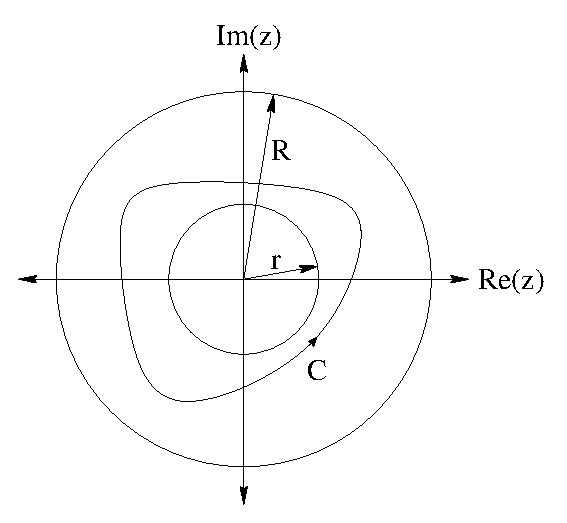
\includegraphics[width=0.4\textwidth]{appendix/app_path_int}
  \end{center}
  \caption{The Path of Integration.}
  \label{app_path_int}
\end{figure}






\raggedbottom
%%===========================================================================
%%===========================================================================
\chapter{Table of Derivatives}
\label{table_of_derivatives}
\raggedbottom 

%% CONTINUE add page references

Note: $c$ denotes a constant and $'$ denotes differentiation.

\setlongtables
\begin{longtable}{l}
  $\displaystyle \frac{\dd}{\dd x} (f g) = \frac{\dd f}{\dd x} g + f \frac{\dd g}{\dd x}$\\
  \\
  $\displaystyle \frac{\dd}{\dd x} \, \frac{f}{g}
  = \frac{f' g - f g'}{g^2}$ \\
  \\
  $\displaystyle \frac{\dd}{\dd x} f^c = c f^{c-1}f'$ \\
  \\
  $\displaystyle \frac{\dd}{\dd x} f(g) = f'(g) g'$ \\
  \\
  $\displaystyle \frac{\dd^2}{\dd x^2} f(g) = f''(g) (g')^2 + f' g''$ \\
  \\
  $\displaystyle \frac{\dd^n}{\dd x^n}(f g) 
  = \binom{n}{0} \frac{\dd^n f}{\dd x^n} g + 
  \binom{n}{1} \frac{\dd^{n-1} f}{\dd x^{n-1}} \frac{\dd g}{\dd x} + 
  \binom{n}{2} \frac{\dd^{n-2} f}{\dd x^{n-2}} \frac{\dd^2 g}{\dd x^2} + \cdots + 
  \binom{n}{n} f \frac{\dd^n g}{\dd x^n}$ \\
  \\
  $\displaystyle \frac{\dd}{\dd x} \ln x = \frac{1}{|x|}$ \\
  \\
  $\displaystyle \frac{\dd}{\dd x} c^x = c^x \ln c$ \\
  \\
  $\displaystyle \frac{\dd}{\dd x} f^g = g f^{g-1} \frac{\dd f}{\dd x}
  + f^g \ln f \frac{\dd g}{\dd x}$ \\
  \\
  $\displaystyle \frac{\dd}{\dd x} \sin x = \cos x$ \\
  \\
  $\displaystyle \frac{\dd}{\dd x} \cos x = - \sin x$ \\
  \\
  $\displaystyle \frac{\dd}{\dd x} \tan x = \sec^2 x$ \\
  \\
  $\displaystyle \frac{\dd}{\dd x} \csc x = - \csc x \cot x$ \\
  \\
  $\displaystyle \frac{\dd}{\dd x} \sec x = \sec x \tan x$ \\
  \\
  $\displaystyle \frac{\dd}{\dd x} \cot x = - \csc^2 x$ \\ 
  \\
  $\displaystyle \frac{\dd}{\dd x} \arcsin x = \frac{1}{\sqrt{1-x^2}}, \qquad
  -\frac{\pi}{2} \leq \arcsin x \leq \frac{\pi}{2}$ \\
  \\
  $\displaystyle \frac{\dd}{\dd x} \arccos x = - \frac{1}{\sqrt{1-x^2}}, \qquad
  0 \leq \arccos x \leq \pi$ \\
  \\
  $\displaystyle \frac{\dd}{\dd x} \arctan x = \frac{1}{1+x^2}, \qquad
  -\frac{\pi}{2} \leq \arctan x \leq \frac{\pi}{2}$ \\
  \\
  $\displaystyle \frac{\dd}{\dd x} \sinh x = \cosh x$ \\
  \\
  $\displaystyle \frac{\dd}{\dd x} \cosh x = \sinh x$ \\
  \\
  $\displaystyle \frac{\dd}{\dd x} \tanh x = \sech^2 x$ \\
  \\
  $\displaystyle \frac{\dd}{\dd x} \csch x = - \csch x \coth x$ \\
  \\
  $\displaystyle \frac{\dd}{\dd x} \sech x = - \sech x \tanh x$ \\
  \\
  $\displaystyle \frac{\dd}{\dd x} \coth x = - \csch^2 x$ \\
  \\
  $\displaystyle \frac{\dd}{\dd x} \arcsinh x = \frac{1}{\sqrt{x^2+1}}$ \\
  \\
  $\displaystyle \frac{\dd}{\dd x} \arccosh x = \frac{1}{\sqrt{x^2-1}}, \qquad
  x > 1,\ \arccosh x > 0$ \\
  \\
  $\displaystyle \frac{\dd}{\dd x} \arctanh x = \frac{1}{1-x^2}, \qquad
  x^2 < 1$ \\
  \\
  $\displaystyle \frac{\dd}{\dd x} \int_c^x f(\xi)\,d\xi = f(x)$ \\
  \\
  $\displaystyle \frac{\dd}{\dd x} \int_x^c f(\xi)\,d\xi = - f(x)$ \\
  \\
  $\displaystyle \frac{\dd}{\dd x} \int_g^h f(\xi,x)\,d\xi 
  = \int_g^h \frac{\partial f(\xi,x)}{\partial x}\,d\xi + f(h,x) h' - f(g,x) g'$
\end{longtable}










\raggedbottom
%%===========================================================================
%%===========================================================================
\chapter{Table of Integrals}
\label{table_of_integrals}
\raggedbottom 

\setlongtables
\begin{longtable}{l}
  $\displaystyle \int u \frac{\dd v}{\dd x}\,d x = u v - \int v \frac{\dd u}{\dd x}\,d x$ \\
  \\
  $\displaystyle \int \frac{f'(x)}{f(x)}\,d x = \log f(x)$ \\
  \\
  $\displaystyle \int \frac{f'(x)}{2 \sqrt{f(x)}}\,d x = \sqrt{f(x)}$ \\
  \\
  $\displaystyle \int x^\alpha\,d x = \frac{x^{\alpha+1}}{\alpha+1} 
  \qquad \mathrm{for}\ \alpha \neq = -1$ \\
  \\
  $\displaystyle \int \frac{1}{x}\,d x = \log x$ \\
  \\
  $\displaystyle \int \e^{a x}\,d x = \frac{\e^{a x}}{a}$ \\
  \\
  $\displaystyle \int a^{b x}\,d x = \frac{a^{b x}}{b \log a} 
  \qquad \mathrm{for}\ a > 0$ \\
  \\
  $\displaystyle \int \log x\,d x = x \log x - x$ \\
  \\
  $\displaystyle \int \frac{1}{x^2 + a^2}\,d x 
  = \frac{1}{a} \arctan \frac{x}{a}$ \\
  \\
  $\displaystyle \int \frac{1}{x^2-a^2}\,d x = 
  \begin{cases}
    \frac{1}{2a} \log \frac{a-x}{a+x} \quad &\mathrm{for}\ x^2 < a^2 \\
    \frac{1}{2a} \log \frac{x-a}{x+a} \quad &\mathrm{for}\ x^2 > a^2
  \end{cases}$ \\
  \\
  $\displaystyle \int \frac{1}{\sqrt{a^2-x^2}}\,d x = \arcsin \frac{x}{|a|} 
  = - \arccos \frac{x}{|a|} \qquad \mathrm{for}\  x^2 < a^2$ \\
  \\
  $\displaystyle \int \frac{1}{\sqrt{x^2 \pm a^2}}\,d x 
  = \log (x + \sqrt{x^2 \pm a^2})$ \\
  \\
  $\displaystyle \int \frac{1}{x \sqrt{x^2 - a^2}}\,d x 
  = \frac{1}{|a|} \sec^{-1} \frac{x}{a}$ \\
  \\
  $\displaystyle \int \frac{1}{x \sqrt{a^2 \pm x^2}}\,d x 
  = - \frac{1}{a} \log \left(
    \frac{a + \sqrt{a^2 \pm x^2}}{x} \right)$ \\
  \\
  $\displaystyle \int \sin(a x)\,d x = - \frac{1}{a} \cos (a x)$ \\
  \\
  $\displaystyle \int \cos(a x)\,d x = \frac{1}{a} \sin (a x)$ \\
  \\
  $\displaystyle \int \tan(a x)\,d x = - \frac{1}{a} \log \cos (a x)$ \\
  \\
  $\displaystyle \int \csc(a x)\,d x = \frac{1}{a} \log \tan \frac{a x}{2}$ \\
  \\
  $\displaystyle \int \sec(a x)\,d x 
  = \frac{1}{a} \log \tan \left( \frac{\pi}{4} + \frac{a x}{2}
  \right)$\\
  \\
  $\displaystyle \int \cot(a x)\,d x = \frac{1}{a} \log \sin (a x)$ \\
  \\
  $\displaystyle \int \sinh(a x)\,d x = \frac{1}{a} \cosh (a x)$ \\
  \\
  $\displaystyle \int \cosh(a x)\,d x = \frac{1}{a} \sinh (a x)$ \\
  \\
  $\displaystyle \int \tanh(a x)\,d x = \frac{1}{a} \log \cosh (a x)$ \\
  \\
  $\displaystyle \int \csch(a x)\,d x = \frac{1}{a} \log \tanh \frac{a x}{2}$ \\
  \\
  $\displaystyle \int \sech(a x)\,d x 
  = \frac{i}{a} \log \tanh \left( \frac{i \pi}{4} +
    \frac{a x}{2} \right)$ \\
  \\
  $\displaystyle \int \coth(a x)\,d x = \frac{1}{a} \log \sinh (a x)$ \\
  \\
  $\displaystyle \int x \sin a x\,d x 
  = \frac{1}{a^2} \sin a x - \frac{x}{a} \cos a x$ \\
  \\
  $\displaystyle \int x^2 \sin a x\,d x 
  = \frac{2x}{a^2} \sin a x - \frac{a^2 x^2-2}{a^3} \cos a x$ \\
  \\
  $\displaystyle \int x \cos a x\,d x 
  = \frac{1}{a^2} \cos a x + \frac{x}{a} \sin a x$ \\
  \\
  $\displaystyle \int x^2 \cos a x\,d x 
  = \frac{2x \cos a x}{a^2} + \frac{a^2 x^2 - 2}{a^3} \sin a x$
\end{longtable}









\raggedbottom
%%===========================================================================
%%===========================================================================
\chapter{Definite Integrals}
\label{definite_integrals}
\flushbottom


\paragraph{Integrals from $\boldsymbol{-} \boldsymbol{\infty}$ 
to $\boldsymbol{\infty}$.}
Let $f(z)$ be analytic except for isolated singularities, none of which
lie on the real axis.
Let $a_1,\ldots,a_m$ be the singularities of $f(z)$ in the upper half plane;
and $C_R$ be the semi-circle from $R$ to $-R$ in the upper half plane.
If
\[
\lim_{R \to \infty} \left( R \max_{z \in C_R} |f(z)| \right) = 0
\]
then
\[
\int_{-\infty}^\infty f(x) \,d x = \imath 2 \pi \sum_{j=1}^m \Res \left( f(z), a_j \right).
\]
Let $b_1,\ldots,b_n$ be the singularities of $f(z)$ in the lower half plane.
Let $C_R$ be the semi-circle from $R$ to $-R$ in the lower half plane.
If
\[
\lim_{R \to \infty} \left( R \max_{z \in C_R} |f(z)| \right) = 0
\]
then
\[
\int_{-\infty}^\infty f(x) \,d x = - \imath 2 \pi \sum_{j=1}^n \Res \left( f(z), b_j \right).
\]





\paragraph{Integrals from $\mathbf{0}$ to $\boldsymbol{\infty}$.}
Let $f(z)$ be analytic except for isolated singularities, none of which
lie on the positive real axis, $[0,\infty)$.
Let $z_1,\ldots,z_n$ be the singularities of $f(z)$.
If $f(z) \ll z^\alpha$ as $z \to 0$ for some $\alpha > -1$ and 
$f(z) \ll z^\beta$ as $z \to \infty$ for some $\beta < -1$ then
\[
\int_0^\infty f(x)\,d x = - \sum_{k = 1}^n \Res \left( f(z) \log z, z_k \right).
\]
\[
\int_0^\infty f(x) \log \,d x
= - \frac{1}{2} \sum_{k=1}^n \Res \left( f(z) \log^2 z, z_k \right)
+ \imath \pi \sum_{k=1}^n \Res \left( f(z) \log z, z_k \right)
\]
Assume that $a$ is not an integer.
If $z^a f(z) \ll z^\alpha$ as $z \to 0$ for some $\alpha > -1$ and 
$z^a f(z) \ll z^\beta$ as $z \to \infty$ for some $\beta < -1$ then
\[
\int_0^\infty x^a f(x)\,d x = \frac{ \imath 2 \pi }{ 1 - \e^{\imath 2 \pi a} } 
\sum_{k = 1}^n \Res \left( z^a f(z), z_k \right).
\]
\[
\int_0^\infty x^a f(x) \log x \,d x
= \frac{ \imath 2 \pi }{ 1 - \e^{\imath 2 \pi a} }
\sum_{k=1}^n \Res \left( z^a f(z) \log z, z_k \right),
+ \frac{ \pi^2 a }{ \sin^2 (\pi a) }
\sum_{k=1}^n \Res \left( z^a f(z), z_k \right)
\]




\paragraph{Fourier Integrals.}
Let $f(z)$ be analytic except for isolated singularities, none
of which lie on the real axis.  Suppose that $f(z)$ vanishes as 
$|z| \to \infty$.  If $\omega$ is a positive real number then
\[
\int_{-\infty}^\infty f(x) \e^{\imath \omega x} \,d x
= \imath 2 \pi \sum_{k = 1}^n \Res( f(z) \e^{\imath \omega z}, z_k ),
\]
where $z_1, \ldots, z_n$ are the singularities of $f(z)$ in the upper
half plane.
If $\omega$ is a negative real number then
\[
\int_{-\infty}^\infty f(x) \e^{\imath \omega x} \,d x
= - \imath 2 \pi \sum_{k = 1}^n \Res( f(z) \e^{\imath \omega z}, z_k ),
\]
where $z_1, \ldots, z_n$ are the singularities of $f(z)$ in the lower
half plane.



%% CONTINUE: Fourier Sine and Cosine integrals


%% CONTINUE: Add a chapter on infinite sums.





\raggedbottom
%%===========================================================================
%%===========================================================================
\chapter{Table of Sums}
\raggedbottom 





\setlongtables
\begin{longtable}{l}
  $\displaystyle \sum_{n = 1}^\infty r^n = \frac{r}{1-r}, \quad \mathrm{for}\  |r| < 1$ \\
  \\
  $\displaystyle \sum_{n=1}^N r^n = \frac{r-r^{N+1}}{1-r}$ \\
  \\
  $\displaystyle \sum_{n=a}^b n = \frac{(a+b)(b+1-a)}{2}$ \\
  \\
  $\displaystyle \sum_{n=1}^N n = \frac{N(N+1)}{2}$ \\
  \\
  $\displaystyle \sum_{n=a}^b n^2 = \frac{b(b+1)(2b+1)-a(a-1)(2a-1)}{6}$ \\
  \\
  $\displaystyle \sum_{n=1}^N n^2 = \frac{N(N+1)(2N+1)}{6}$ \\
  \\
  $\displaystyle \sum_{n = 1}^\infty \frac{(-1)^{n+1}}{n} = \log(2)$ \\
  \\
  $\displaystyle \sum_{n = 1}^\infty \frac{1}{n^2} = \frac{\pi^2}{6}$ \\
  \\
  $\displaystyle \sum_{n = 1}^\infty \frac{(-1)^{n+1}}{n^2} = \frac{\pi^2}{12}$ \\
  \\
  $\displaystyle \sum_{n = 1}^\infty \frac{1}{n^3} = \zeta(3)$ \\
  \\
  $\displaystyle \sum_{n = 1}^\infty \frac{(-1)^{n+1}}{n^3} = \frac{3 \zeta(3)}{4}$ \\
  \\
  $\displaystyle \sum_{n = 1}^\infty \frac{1}{n^4} = \frac{\pi^4}{90}$ \\
  \\
  $\displaystyle \sum_{n = 1}^\infty \frac{(-1)^{n+1}}{n^4} = \frac{7 \pi^4}{720}$ \\
  \\
  $\displaystyle \sum_{n = 1}^\infty \frac{1}{n^5} = \zeta(5)$ \\
  \\
  $\displaystyle \sum_{n = 1}^\infty \frac{(-1)^{n+1}}{n^5} = \frac{15 \zeta(5)}{16}$ \\
  \\
  $\displaystyle \sum_{n = 1}^\infty \frac{1}{n^6} = \frac{\pi^6}{945}$ \\
  \\
  $\displaystyle \sum_{n = 1}^\infty \frac{(-1)^{n+1}}{n^6} = \frac{31 \pi^6}{30240}$
\end{longtable}








\raggedbottom
%%============================================================================
%%============================================================================
\chapter{Table of Taylor Series}
\label{table_of_taylor_series}
\index{Taylor series!table of}
\raggedbottom 


\setlongtables
\begin{longtable}{ll}
  $\displaystyle (1 - z)^{-1} = \sum_{n = 0}^\infty z^n$ & $|z| < 1$ \\
  \\
  $\displaystyle (1 - z)^{-2} = \sum_{n = 0}^\infty (n+1)z^n$ & $|z| < 1$ \\
  \\
  $\displaystyle (1 + z)^\alpha = \sum_{n = 0}^\infty \binom{\alpha}{n}z^n$ & $|z| < 1$ \\
  \\
  $\displaystyle \e^z = \sum_{n = 0}^\infty \frac{z^n}{n!}$ & $|z| < \infty$ \\
  \\
  $\displaystyle \log(1-z) = -\sum_{n=1}^\infty \frac{z^n}{n}$ & $|z| < 1$ \\
  \\
  $\displaystyle \log \left(\frac{1+z}{1-z}\right) 
  = 2 \sum_{n = 1}^\infty \frac{z^{2n-1}}{2n-1}$ & $|z| < 1$ \\
  \\
  $\displaystyle \cos z = \sum_{n = 0}^\infty \frac{(-1)^n z^{2n}}{(2n)!}$
  & $|z| < \infty$ \\
  \\
  $\displaystyle \sin z = \sum_{n = 0}^\infty \frac{(-1)^n z^{2n+1}}{(2n+1)!}$
  & $|z| < \infty$ \\
  \\
  $\displaystyle \tan z = z + \frac{z^3}{3} + \frac{2 z^5}{15} 
  + \frac{17 z^7}{315} + \cdots$ & $|z| < \frac{\pi}{2}$ \\
  \\
  $\displaystyle \cos^{-1} z = \frac{\pi}{2} - \left( z + \frac{z^3}{2 \cdot 3} 
    + \frac{1 \cdot 3 z^5}{2 \cdot 4 \cdot 5}
    + \frac{1 \cdot 3 \cdot 5 z^7}{2 \cdot 4 \cdot 6 \cdot 7}
    + \cdots \right)$ & $|z| < 1$ \\
  \\
  $\displaystyle \sin^{-1} z = z + \frac{z^3}{2 \cdot 3} 
  + \frac{1 \cdot 3 z^5}{2 \cdot 4 \cdot 5}
  + \frac{1 \cdot 3 \cdot 5 z^7}{2 \cdot 4 \cdot 6 \cdot 7}
  + \cdots$  & $|z| < 1$ \\
  \\
  $\displaystyle \tan^{-1} z = \sum_{n = 1}^\infty \frac{(-1)^{n+1} z^{2n-1}}{2n-1}$
  & $|z| < 1$ \\
  \\
  $\displaystyle \cosh z = \sum_{n = 0}^\infty \frac{z^{2n}}{(2n)!}$ & $|z| < \infty$ \\
  \\
  $\displaystyle \sinh z = \sum_{n = 0}^\infty \frac{z^{2n+1}}{(2n+1)!}$ 
  & $|z| < \infty$ \\
  \\
  $\displaystyle \tanh z = z - \frac{z^3}{3} + \frac{2 z^5}{15} 
  - \frac{17 z^7}{315} + \cdots$ & $|z| < \frac{\pi}{2}$ \\
  \\
  $\displaystyle J_\nu(z) = \sum_{n = 0}^\infty \frac{(-1)^n}{n! \Gamma(\nu + n + 1)} 
  \left( \frac{z}{2} \right)^{\nu + 2n}$ & $|z| < \infty$ \\
  \\
  $\displaystyle I_\nu(z) = \sum_{n = 0}^\infty \frac{1}{n! \Gamma(\nu + n + 1)} 
  \left( \frac{z}{2}\right)^{\nu + 2n}$ & $|z| < \infty$ 
\end{longtable}













\raggedbottom
%%=============================================================================
%%=============================================================================
\chapter{Continuous Transforms}
\raggedbottom 


%%=============================================================================
\section{Properties of Laplace Transforms}


Let $f(t)$ be piecewise continuous and of exponential order $\alpha$.
Unless otherwise noted, the transform is defined for $s > 0$.
To reduce clutter, it is understood that the Heaviside function $H(t)$
multiplies the original function in the following two tables.

\setlongtables
\begin{longtable}{lll}
  $\displaystyle \mathbf{f \boldsymbol{(} t \boldsymbol{)}}$
  & $\displaystyle \mathbf{\boldsymbol{\int}_0^{\boldsymbol{\infty}} \e^{-s t}f \boldsymbol{(} t \boldsymbol{)} \,dt}$ 
  & \\
  \\
  $\displaystyle \frac{1}{\imath 2 \pi} 
  \int_{c - \imath \infty}^{c + \imath \infty} \e^{t s} \hat{f}(s)\,d s$
  & $\displaystyle \hat{f}(s)$ 
  & \\
  \\
  $\displaystyle a f(t) + b g(t)$
  & $\displaystyle a \hat{f}(s) + b \hat{g}(s)$ 
  & \\
  \\
  $\displaystyle \frac{\dd}{\dd t} f(t)$
  & $\displaystyle s \hat{f}(s) - f(0)$
  & \\
  \\
  $\displaystyle \frac{\dd^2}{\dd t^2} f(t)$
  & $\displaystyle s^2 \hat{f}(s) - s f(0) - f'(0)$
  & \\
  \\
  $\displaystyle \frac{\dd^n}{\dd t^n} f(t)$
  & $\displaystyle s^n \hat{f}(s) - s^{n-1} f(0)$
  & \\
  %%
  & $\quad - s^{n-2} f'(0) - \cdots - f^{(n-1)}(0)$
  & \\
  \\
  $\displaystyle \int_0^t f(\tau)\,d\tau$
  & $\displaystyle \frac{\hat{f}(s)}{s}$
  & \\
  \\
  $\displaystyle \int_0^t \int_0^\tau f(s)\,ds\,d\tau$
  & $\displaystyle \frac{\hat{f}(s)}{s^2}$
  & \\
  \\
  $\displaystyle \e^{c t} f(t)$
  & $\displaystyle \hat{f}(s - c)$
  & $s > c + \alpha$ \\
  \\
  $\displaystyle \frac{1}{c} f \left( \frac{t}{c} \right), \quad c > 0$
  & $\displaystyle \hat{f}(c s)$
  & \\
  \\
  $\displaystyle \frac{1}{c} \e^{(b / c) t} f \left( \frac{t}{c} \right),\quad c > 0$
  & $\displaystyle \hat{f}(c s - b)$
  & \\
  \\
  $\displaystyle f(t - c) H(t - c), \quad c > 0$
  & $\displaystyle \e^{- c s} \hat{f}(s)$
  & \\ %% CONTINUE: CHECK THE RANGE
  \\
  $\displaystyle t f(t)$
  & $\displaystyle -\frac{\dd}{\dd s} \hat{f}(s)$
  & \\
  \\
  $\displaystyle t^n f(t)$
  & $\displaystyle (-1)^n \frac{\dd^n}{\dd s^n} \hat{f}(s)$
  & \\
  \\
  $\displaystyle \frac{f(t)}{t}, 
  \quad \int_0^1 \frac{f(t)}{t}\,\dd t \ \mathrm{exists}$
  & $\displaystyle \int_s^\infty \hat{f}(t)\,\dd t$
  & \\
  \\
  $\displaystyle \int_0^t f(\tau)g(t - \tau)\,\dd \tau, 
  \quad f,g \in C^0$
  & $\displaystyle \hat{f}(s) \hat{g}(s)$
  & \\
  \\
  $\displaystyle f(t), \quad f(t + T) = f(t)$
  & $\displaystyle \frac{\int_0^T \e^{- s t} f(t)\,\dd t}{1 - \e^{- s T}}$
  & \\
  \\
  $\displaystyle f(t), \quad f(t + T) = - f(t)$
  & $\displaystyle \frac{\int_0^T \e^{- s t} f(t)\,\dd t}{1 + \e^{- s T}}$
  & 
\end{longtable}







%%=============================================================================
\pagebreak
\section{Table of Laplace Transforms}



\setlongtables
\begin{longtable}{lll}
  $\displaystyle \mathbf{f \boldsymbol{(} t \boldsymbol{)}}$
  & $\displaystyle \mathbf{\boldsymbol{\int}_0^{\boldsymbol{\infty}} \e^{-s t}f \boldsymbol{(} t \boldsymbol{)} \,dt}$ 
  & \\
  \\
  $\displaystyle \frac{1}{\imath 2 \pi} 
  \int_{c - \imath \infty}^{c + \imath \infty} \e^{t s} \hat{f}(s)\,d s$
  & $\displaystyle \hat{f}(s)$ 
  & \\
  \\
  $\displaystyle 1$
  & $\displaystyle \frac{1}{s}$
  & \\
  \\
  $\displaystyle t$
  & $\displaystyle \frac{1}{s^2}$
  & \\
  \\
  $\displaystyle t^n,\ \mathrm{for}\ n = 0,1,2,\ldots$
  & $\displaystyle \frac{n!}{s^{n+1}}$
  & \\
  \\
  $\displaystyle t^{1/2}$
  & $\displaystyle \frac{\sqrt{\pi}}{2} s^{-3/2}$
  & \\
  \\
  $\displaystyle t^{-1/2}$
  & $\displaystyle \sqrt{\pi} s^{-1/2}$
  & \\
  \\
  $\displaystyle t^{n-1/2}, \quad n \in \mathbb{Z}^+$
  & $\displaystyle \frac{(1) (3) (5) \cdots
    (2n-1) \sqrt{\pi}}{2^n} s^{-n-1/2}$
  & \\
  \\
  $\displaystyle t^\nu, \quad \Re(\nu) > -1$
  & $\displaystyle \frac{\Gamma(\nu+1)}{s^{\nu+1}}$
  & \\
  \\
  $\displaystyle \Log t$
  & $\displaystyle \frac{-\gamma - \Log s}{s}$
  & \\
  \\
  $\displaystyle t^\nu \Log t, \quad \Re(\nu) > -1$
  & $\displaystyle \frac{\Gamma(\nu+1)}{s^{n+1}} (\psi(\nu+1) - \Log s)$
  & \\
  \\
  $\displaystyle \delta(t)$
  & $\displaystyle 1$
  & $s > 0$ \\
  \\
  $\displaystyle \delta^{(n)}(t), \quad n \in \mathbb{Z}^{0+}$
  & $\displaystyle s^n$
  & $s > 0$ \\
  \\
  $\displaystyle \e^{c t}$
  & $\displaystyle \frac{1}{s-c}$
  & $s > c$
  \\
  $\displaystyle t \e^{c t}$
  & $\displaystyle \frac{1}{(s-c)^2}$
  & $s > c$ \\
  \\
  $\displaystyle \frac{t^{n-1} \e^{c t}}{(n-1)!}, 
  n \in \mathbb{Z}^+$
  & $\displaystyle \frac{1}{(s-c)^n}$
  & $s > c$ \\
  \\
  $\displaystyle \sin(c t)$
  & $\displaystyle \frac{c}{s^2 + c^2}$
  & \\
  \\
  $\displaystyle \cos(c t)$
  & $\displaystyle \frac{s}{s^2 + c^2}$
  & \\
  \\
  $\displaystyle \sinh(c t)$
  & $\displaystyle \frac{c}{s^2-c^2}$
  & $s > |c|$ \\
  \\
  $\displaystyle \cosh(c t)$
  & $\displaystyle \frac{s}{s^2 - c^2}$
  & $s > |c|$ \\
  \\
  $\displaystyle t \sin(c t)$
  & $\displaystyle \frac{2c s}{(s^2 + c^2)^2}$
  & \\
  \\
  $\displaystyle t \cos(c t)$
  & $\displaystyle \frac{s^2 - c^2}{(s^2+c^2)^2}$
  & \\
  \\
  $\displaystyle t^n \e^{c t} , \quad n \in \mathbb{Z}^+$
  & $\displaystyle \frac{n!}{(s-c)^{n+1}}$
  & \\
  \\
  $\displaystyle \e^{d t} \sin(c t)$
  & $\displaystyle \frac{c}{(s-d)^2 + c^2}$
  & $s > d$ \\
  \\
  $\displaystyle \e^{d t} \cos(c t)$
  & $\displaystyle \frac{s - d}{(s-d)^2+c^2}$
  & $s > d$ \\
  \\
  $\displaystyle \delta(t-c)$
  & $\displaystyle \begin{cases}
    0 \quad &\mathrm{for}\  c < 0 \\
    \e^{-s c} \quad &\mathrm{for}\ c > 0
  \end{cases}$
  & \\
  \\
  $\displaystyle H(t-c) = \begin{cases}
    0 \quad &\mathrm{for}\ t < c \\
    1 \quad &\mathrm{for}\ t > c
  \end{cases}$
  & $\displaystyle \frac{1}{s}\e^{-c s}$
  & \\
  \\
  $\displaystyle J_\nu(c t)$
  & $\displaystyle \frac{c^n}{\sqrt{s^2 + c^2} 
    \left( s + \sqrt{s^2 + c^2} \right)^\nu}$
  & $\nu > -1$ \\
  \\
  $\displaystyle I_\nu(c t)$
  & $\displaystyle \frac{c^n}{\sqrt{s^2 - c^2} 
    \left( s - \sqrt{s^2 + c^2} \right)^\nu}$
  & $\Re(s) > c$, $\nu > -1$
\end{longtable}










%%============================================================================
\pagebreak
\section{Table of Fourier Transforms}
\index{Fourier transform!table of}

\setlongtables
\begin{longtable}{ll}
  $\displaystyle \mathbf{f  \boldsymbol{(} x \boldsymbol{)}}$
  & $\displaystyle \mathbf{\frac{1}{2 \boldsymbol{\pi}} 
    \boldsymbol{\int}_{-\boldsymbol{\infty}}^{\boldsymbol{\infty}} f \boldsymbol{(} x \boldsymbol{)}  
    \e^{- \boldsymbol{\imath} \boldsymbol{\omega} x}\,\dd x }$ \\
  \\
  $\displaystyle \mathbf{\boldsymbol{\int}_{-\boldsymbol{\infty}}^{\boldsymbol{\infty}} 
    F \boldsymbol{(} \boldsymbol{\omega} \boldsymbol{)} \e^{\boldsymbol{\imath} \boldsymbol{\omega} x} \,\dd \boldsymbol{\omega} }$
  & $\displaystyle \mathbf{ F \boldsymbol{(} \omega \boldsymbol{)}}$ \\
  \\
  $\displaystyle a f(x) + b g(x)$
  & $\displaystyle a F(\omega) + b G(\omega)$ \\
  \\
  $\displaystyle f^{(n)}(x)$
  & $\displaystyle (\imath \omega)^n F(\omega)$ \\
  \\
  $\displaystyle x^n f(x)$
  & $\displaystyle \imath^n F^{(n)}(\omega)$ \\
  \\
  $\displaystyle f(x + c)$
  & $\displaystyle \e^{\imath \omega c} F(\omega)$ \\
  \\
  $\displaystyle \e^{- \imath c x} f(x)$
  & $\displaystyle F(\omega + c)$ \\
  \\
  $\displaystyle f(c x)$
  & $\displaystyle |c|^{-1} F(\omega/c)$ \\
  \\
  $\displaystyle f(x) g(x)$
  & $\displaystyle F * G(\omega) = \int_{-\infty}^\infty F(\eta) G(\omega - \eta)\,\dd \eta$ \\
  \\
  $\displaystyle \frac{1}{2\pi} f * g(x) = \frac{1}{2 \pi} 
  \int_{-\infty}^\infty f(\xi)g(x - \xi)\,\dd \xi$
  & $\displaystyle F(\omega) G(\omega)$ \\
  \\
  $\displaystyle \e^{-c x^2}, \quad c > 0$
  & $\displaystyle \frac{1}{\sqrt{4 \pi c}} \e^{-\omega^2/4c}$ \\
  \\
  $\displaystyle \e^{-c |x|}, \quad c > 0$
  & $\displaystyle \frac{c / \pi}{\omega^2 + c^2}$ \\
  \\
  $\displaystyle \frac{2 c}{x^2 + c^2}, \quad c > 0$
  & $\displaystyle \e^{-c |\omega|}$ \\
  \\
  $\displaystyle \frac{1}{x - \imath \alpha}, \quad \alpha > 0$
  & $\displaystyle \begin{cases}
    0 \quad &\mathrm{for}\ \omega > 0 \\
    \imath \e^{\alpha \omega} \quad &\mathrm{for}\ \omega < 0
  \end{cases}$ \\
  \\
  $\displaystyle \frac{1}{x - \imath \alpha}, \quad \alpha < 0$
  & $\displaystyle \begin{cases}
    \imath \e^{\alpha \omega} \quad &\mathrm{for}\ \omega > 0 \\
    0 \quad &\mathrm{for}\  \omega < 0
  \end{cases}$ \\
  \\
  $\displaystyle \frac{1}{x}$
  & $\displaystyle -\frac{\imath}{2} \sign(\omega)$ \\
  \\
  $\displaystyle H(x - c) = \begin{cases}
    0 \quad &\mathrm{for}\ x < c \\
    1 \quad &\mathrm{for}\ x > c
  \end{cases}$
  & $\displaystyle \frac{1}{\imath 2 \pi \omega} \e^{- \imath c \omega}$ \\
  \\
  $\displaystyle \e^{- c x} H(x),\quad \Re(c) > 0$
  & $\displaystyle \frac{ 1 }{ 2 \pi (c + \imath \omega) }$ \\
  \\
  $\displaystyle \e^{c x} H(- x),\quad \Re(c) > 0$
  & $\displaystyle \frac{ 1 }{ 2 \pi (c - \imath \omega) }$ \\
  \\
  $\displaystyle 1$
  & $\displaystyle \delta(\omega)$ \\
  \\
  $\displaystyle \delta(x - \xi)$
  & $\displaystyle \frac{1}{2 \pi} \e^{- \imath \omega \xi}$ \\
  \\
  $\displaystyle \pi( \delta(x + \xi) + \delta(x - \xi) )$
  & $\displaystyle \cos(\omega \xi)$ \\
  \\
  $\displaystyle - \imath \pi( \delta(x + \xi) - \delta(x - \xi) )$
  & $\displaystyle \sin(\omega \xi)$ \\
  \\
  $\displaystyle H(c - |x|) = \begin{cases}
    1 \quad &\mathrm{for}\ |x| < c \\
    0 \quad &\mathrm{for}\ |x| > c 
  \end{cases}$,\ $c > 0$
  & $\displaystyle \frac{\sin(c \omega)}{\pi \omega}$
\end{longtable}











%%============================================================================
\pagebreak
\section{Table of Fourier Transforms in n Dimensions}
\index{Fourier transform!table of}


\setlongtables
\begin{longtable}{ll}
  $\displaystyle \mathbf{f  \boldsymbol{(} x \boldsymbol{)}}$
  &
  $\displaystyle \mathbf{\frac{1}{\boldsymbol{(} 2\boldsymbol{\pi} \boldsymbol{)}^n} 
    \boldsymbol{\int}_{\mathbb{R}^n} f \boldsymbol{(} x \boldsymbol{)}  \e^{-\boldsymbol{\imath} \boldsymbol{\omega} x}\,\dd x }$ \\
  \\
  %%
  $\displaystyle \mathbf{\boldsymbol{\int}_{\mathbb{R}^n} F \boldsymbol{(} \boldsymbol{\omega} \boldsymbol{)} 
    \e^{\boldsymbol{\imath} \boldsymbol{\omega} x} \,\dd\boldsymbol{\omega} }$
  &
  $\displaystyle \mathbf{ F \boldsymbol{(} \omega \boldsymbol{)}}$  \\
  \\
  %%
  $\displaystyle a f(x) + b g(x)$
  &
  $\displaystyle a F(\omega) + b G(\omega)$ \\
  \\
  %%
  $\displaystyle \left( \frac{\pi}{c} \right)^{n/2} \e^{-n x^2 / 4c}$
  &
  $\displaystyle \e^{-c \omega^2}$
\end{longtable}



%% CONTINUE









%%============================================================================
\pagebreak
\section{Table of Fourier Cosine Transforms}
\index{Fourier cosine transform!table of}

%%FourierParameters -> {-1, -1}
\setlongtables
\begin{longtable}{ll}
  $\displaystyle \mathbf{f \boldsymbol{(} x \boldsymbol{)}}$
  & $\displaystyle \mathbf{\frac{1}{\boldsymbol{\pi}} \boldsymbol{\int}_0^{\boldsymbol{\infty}} f \boldsymbol{(} x\boldsymbol{)} 
    \bcos \boldsymbol{(} \boldsymbol{\omega} x \boldsymbol{)} \,d x}$ \\
  \\
  $\displaystyle \mathbf{2 \boldsymbol{\int}_0^{\boldsymbol{\infty}} C \boldsymbol{(} \boldsymbol{\omega}\boldsymbol{)}
    \bcos\boldsymbol{(} \boldsymbol{\omega} x \boldsymbol{)} \,d \boldsymbol{\omega}}$
  & $\displaystyle \mathbf{C \boldsymbol{(} \boldsymbol{\omega} \boldsymbol{)} }$ \\
  \\
  $\displaystyle f'(x)$
  & $\displaystyle \omega S(\omega) - \frac{1}{\pi} f(0)$ \\
  \\
  $\displaystyle f''(x)$
  & $\displaystyle -\omega^2 C(\omega) - \frac{1}{\pi} f'(0)$ \\
  \\
  $\displaystyle x f(x)$
  & $\displaystyle \frac{\partial}{\partial \omega} \mathcal{F}_s [f(x)]$ \\
  \\
  $\displaystyle f(c x), \quad c > 0$
  & $\displaystyle \frac{1}{c} C\left(\frac{\omega}{c}\right)$ \\
  \\
  $\displaystyle \frac{2 c}{x^2 + c^2}$
  & $\displaystyle \e^{- c \omega}$ \\
  \\
  $\displaystyle \e^{-c x}$
  & $\displaystyle \frac{c / \pi}{\omega^2 + c^2}$ \\
  \\
  $\displaystyle \e^{- c x^2}$
  & $\displaystyle \frac{1}{\sqrt{4 \pi c}} \e^{-\omega^2/(4 c)}$ \\
  \\
  $\displaystyle \sqrt{ \frac{\pi}{c} } \e^{-x^2/(4 c)}$
  & $\displaystyle \e^{- c \omega^2}$
\end{longtable}



























%%============================================================================
\pagebreak
\section{Table of Fourier Sine Transforms}
\index{Fourier sine transform!table of}


%%FourierParameters -> {-1, 1}
\setlongtables
\begin{longtable}{ll}
  $\displaystyle \mathbf{f \boldsymbol{(} x \boldsymbol{)} }$
  & $\displaystyle \mathbf{\frac{1}{\boldsymbol{\pi}} \boldsymbol{\int}_0^{\boldsymbol{\infty}} f \boldsymbol{(} x \boldsymbol{)} 
    \bsin \boldsymbol{(} \boldsymbol{\omega} x \boldsymbol{)} \,\dd x}$ \\
  \\
  $\displaystyle \mathbf{2 \boldsymbol{\int}_0^{\boldsymbol{\infty}} S\boldsymbol{(} \boldsymbol{\omega} \boldsymbol{)} 
    \bsin\boldsymbol{(}\boldsymbol{\omega} x \boldsymbol{)}\,\dd \boldsymbol{\omega}}$
  & $\displaystyle \mathbf{S \boldsymbol{(} \boldsymbol{\omega} \boldsymbol{)}}$ \\
  \\
  $\displaystyle f'(x)$
  & $\displaystyle - \omega C(\omega)$ \\
  \\
  $\displaystyle f''(x)$
  & $\displaystyle -\omega^2 S(\omega) + \frac{1}{\pi} \omega f(0)$ \\
  \\
  $\displaystyle x f(x)$
  & $\displaystyle -\frac{\partial}{\partial \omega} \mathcal{F}_c [f(x)]$ \\
  \\
  $\displaystyle f(c x), \quad c > 0$
  & $\displaystyle \frac{1}{c} S\left(\frac{\omega}{c}\right)$ \\
  \\
  $\displaystyle \frac{2x}{x^2 + c^2}$
  & $\displaystyle \e^{-c \omega}$ \\
  \\
  $\displaystyle \e^{-c x}$
  & $\displaystyle \frac{\omega/\pi}{\omega^2 + c^2}$ \\
  \\
  $\displaystyle 2 \arctan \left( \frac{x}{c} \right)$ 
  & $\displaystyle \frac{1}{\omega} \e^{-c \omega}$ \\
  \\
  $\displaystyle \frac{1}{x} \e^{-c x}$
  & $\displaystyle \frac{1}{\pi} \arctan\left( \frac{\omega}{c} \right)$ \\
  \\
  $\displaystyle 1$
  & $\displaystyle \frac{1}{\pi \omega}$ \\
  \\
  $\displaystyle \frac{2}{x}$
  & $\displaystyle 1$ \\
  \\
  $\displaystyle x \e^{-c x^2}$
  & $\displaystyle \frac{\omega}{4 c^{3/2} \sqrt{\pi}} \e^{-\omega^2/(4 c)}$ \\
  \\
  $\displaystyle \frac{\sqrt{\pi} x}{2 c^{3/2}} \e^{-x^2 / (4 c)}$
  & $\displaystyle \omega \e^{-c \omega^2}$
\end{longtable}













\raggedbottom
%%============================================================================
\chapter{Table of Wronskians}
\raggedbottom 


\setlongtables
\begin{longtable}{ll}
  $\displaystyle W \left[ x-a, x-b \right]$
  & $\displaystyle b-a$ \\
  \\
  $\displaystyle W \left[ \e^{a x}, \e^{b x} \right]$
  & $\displaystyle (b-a) \e^{(a+b) x}$ \\
  \\
  $\displaystyle W \left[ \cos(a x), \sin(a x) \right]$
  & $\displaystyle a$ \\
  \\
  $\displaystyle W \left[ \cosh(a x), \sinh(a x) \right]$
  & $\displaystyle a$ \\
  \\
  $\displaystyle W \left[ \e^{a x} \cos(b x), \e^{a x} \sin(b x) \right]$
  & $\displaystyle b \e^{2 a x}$ \\
  \\
  $\displaystyle W \left[ \e^{a x} \cosh(b x), \e^{a x} \sinh(b x) \right]$
  & $\displaystyle b \e^{2 a x}$ \\
  \\
  $\displaystyle W \left[ \sin(c(x-a)), \sin(c(x-b)) \right]$
  & $\displaystyle c \sin(c(b-a))$ \\
  \\
  $\displaystyle W \left[ \cos(c(x-a)), \cos(c(x-b)) \right]$
  & $\displaystyle c \sin(c(b-a))$ \\
  \\
  $\displaystyle W \left[ \sin(c(x-a)), \cos(c(x-b)) \right]$
  & $\displaystyle - c \cos(c(b-a))$ \\
  \\
  $\displaystyle W \left[ \sinh(c(x-a)), \sinh(c(x-b)) \right]$
  & $\displaystyle c \sinh(c(b-a))$ \\
  \\
  $\displaystyle W \left[ \cosh(c(x-a)), \cosh(c(x-b)) \right]$
  & $\displaystyle c \cosh(c(b-a))$ \\
  \\
  $\displaystyle W \left[ \sinh(c(x-a)), \cosh(c(x-b)) \right]$
  & $\displaystyle - c \cosh(c(b-a))$ \\
  \\
  $\displaystyle W \left[ \e^{d x} \sin(c(x-a)), \e^{d x} \sin(c(x-b)) \right]$
  & $\displaystyle c \e^{2 d x} \sin(c (b-a))$ \\
  \\
  $\displaystyle W \left[ \e^{d x} \cos(c(x-a)), \e^{d x} \cos(c(x-b)) \right]$
  & $\displaystyle c \e^{2 d x} \sin(c (b-a))$ \\
  \\
  $\displaystyle W \left[ \e^{d x} \sin(c(x-a)), \e^{d x} \cos(c(x-b)) \right]$
  & $\displaystyle - c \e^{2 d x} \cos(c (b-a))$ \\
  \\
  $\displaystyle W \left[ \e^{d x} \sinh(c(x-a)), \e^{d x} \sinh(c(x-b)) \right]$
  & $\displaystyle c \e^{2 d x} \sinh(c (b-a))$ \\
  \\
  $\displaystyle W \left[ \e^{d x} \cosh(c(x-a)), \e^{d x} \cosh(c(x-b)) \right]$
  & $\displaystyle - c \e^{2 d x} \sinh(c (b-a))$ \\
  \\
  $\displaystyle W \left[ \e^{d x} \sinh(c(x-a)), \e^{d x} \cosh(c(x-b)) \right]$
  & $\displaystyle - c \e^{2 d x} \cosh(c (b-a))$ \\
  \\
  $\displaystyle W \left[ (x-a) \e^{c x}, (x-b) \e^{c x} \right]$
  & $\displaystyle (b-a) \e^{2 c x}$
\end{longtable}















\raggedbottom
%%============================================================================
\chapter{Sturm-Liouville Eigenvalue Problems}
\raggedbottom 


\begin{itemize}
  %%
  %%
\item 
  $y'' + \lambda^2 y = 0$, $y(a) = y(b) = 0$
  \[
  \lambda_n = \frac{n \pi}{b-a}, \quad
  y_n = \sin \left( \frac{n \pi (x-a) }{ b-a } \right), \quad
  n \in \mathbb{N}
  \]
  \[
  \langle y_n, y_n \rangle = \frac{b-a}{2}
  \]
  %%
  %%
\item 
  $y'' + \lambda^2 y = 0$, $y(a) = y'(b) = 0$
  \[
  \lambda_n = \frac{(2n-1) \pi}{2(b-a)}, \quad
  y_n = \sin \left( \frac{(2n-1) \pi (x-a) }{ 2(b-a) } \right), \quad
  n \in \mathbb{N}
  \]
  \[
  \langle y_n, y_n \rangle = \frac{b-a}{2}
  \]
  %%
  %%
\item 
  $y'' + \lambda^2 y = 0$, $y'(a) = y(b) = 0$
  \[
  \lambda_n = \frac{(2n-1) \pi}{2(b-a)}, \quad
  y_n = \cos \left( \frac{(2n-1) \pi (x-a) }{ 2(b-a) } \right), \quad
  n \in \mathbb{N}
  \]
  \[
  \langle y_n, y_n \rangle = \frac{b-a}{2}
  \]
  %%
  %%
\item 
  $y'' + \lambda^2 y = 0$, $y'(a) = y'(b) = 0$
  \[
  \lambda_n = \frac{n \pi}{b-a}, \quad
  y_n = \cos \left( \frac{n \pi (x-a) }{ b-a } \right), \quad
  n = 0,1,2,\ldots
  \]
  \[
  \langle y_0, y_0 \rangle = b-a, \quad
  \langle y_n, y_n \rangle = \frac{b-a}{2}\ \mathrm{for}\ n \in \mathbb{N}
  \]
\end{itemize}
%% CONTINUE


















\raggedbottom
%%============================================================================
\chapter{Green Functions for Ordinary Differential Equations}
\raggedbottom 




\begin{itemize}
  %%
  %%
\item
  $G' + p(x) G = \delta(x-\xi)$, $G(\xi^-:\xi) = 0$
  \[
  G(x|\xi) = \exp \left( - \int_\xi^x p(t) \,\dd t \right) H(x-\xi)
  \]
  %%
  %%
\item
  $y'' = 0$, $y(a) = y(b) = 0$
  \[
  G(x|\xi) = \frac{ (x_< - a) (x_> - b) }
  { b-a }
  \]
  %%
  %%
\item
  $y'' = 0$, $y(a) = y'(b) = 0$
  \[
  G(x|\xi) = a - x_<
  \]
  %%
  %%
\item
  $y'' = 0$, $y'(a) = y(b) = 0$
  \[
  G(x|\xi) = x_> - b
  \]
  %%
  %%
\item
  $y'' - c^2 y = 0$, $y(a) = y(b) = 0$
  \[
  G(x|\xi) = \frac{ \sinh( c (x_< - a) ) \sinh( c (x_> - b) ) }
  { c \sinh( c (b-a) ) }
  \]
  %%
  %%
\item
  $y'' - c^2 y = 0$, $y(a) = y'(b) = 0$
  \[
  G(x|\xi) = - \frac{ \sinh( c (x_< - a) ) \cosh( c (x_> - b) ) }
  { c \cosh( c (b-a) ) }
  \]
  %%
  %%
\item
  $y'' - c^2 y = 0$, $y'(a) = y(b) = 0$
  \[
  G(x|\xi) = \frac{ \cosh( c (x_< - a) ) \sinh( c (x_> - b) ) }
  { c \cosh( c (b-a) ) }
  \]
  %%
  %%
\item
  $y'' + c^2 y = 0$, $y(a) = y(b) = 0$, $c \neq \frac{n pi}{b-a}$, 
  $n \in \mathbb{N}$
  \[
  G(x|\xi) = \frac{ \sin( c (x_< - a) ) \sin( c (x_> - b) ) }
  { c \sin( c (b-a) ) }
  \]
  %%
  %%
\item
  $y'' + c^2 y = 0$, $y(a) = y'(b) = 0$, $c \neq \frac{(2n-1) pi}{2(b-a)}$, 
  $n \in \mathbb{N}$
  \[
  G(x|\xi) = - \frac{ \sin( c (x_< - a) ) \cos( c (x_> - b) ) }
  { c \cos( c (b-a) ) }
  \]
  %%
  %%
\item
  $y'' + c^2 y = 0$, $y'(a) = y(b) = 0$, $c \neq \frac{(2n-1) pi}{2(b-a)}$, 
  $n \in \mathbb{N}$
  \[
  G(x|\xi) = \frac{ \cos( c (x_< - a) ) \sin( c (x_> - b) ) }
  { c \cos( c (b-a) ) }
  \]
  %%
  %%
\item
  $y'' + 2 c y' + d y = 0$, $y(a) = y(b) = 0$, $c^2 > d$
  \[
  G(x|\xi) = \frac{ \e^{-c x_<} \sinh( \sqrt{ c^2 - d } (x_< - a) ) 
    \e^{-c x_<} \sinh( \sqrt{ c^2 - d } (x_> - b) ) }
  { \sqrt{c^2 - d} \e^{-2 c \xi} \sinh( \sqrt{c^2 - d} (b-a) ) }
  \]
  %%
  %%
\item
  $y'' + 2 c y' + d y = 0$, $y(a) = y(b) = 0$, $c^2 < d$, 
  $\sqrt{d - c^2} \neq \frac{n \pi}{b-a}$, $n \in \mathbb{N}$
  \[
  G(x|\xi) = \frac{ \e^{-c x_<} \sin( \sqrt{ d - c^2 } (x_< - a) ) 
    \e^{-c x_<} \sin( \sqrt{ d - c^2 } (x_> - b) ) }
  { \sqrt{d - c^2} \e^{-2 c \xi} \sin( \sqrt{d - c^2} (b-a) ) }
  \]
  %%
  %%
\item
  $y'' + 2 c y' + d y = 0$, $y(a) = y(b) = 0$, $c^2 = d$
  \[
  G(x|\xi) = \frac{ (x_< - a) \e^{-c x_<} (x_> - b) \e^{-c x_<} }
  { (b-a) \e^{-2 c \xi} }
  \]
\end{itemize}


%% CONTINUE











\raggedbottom
%%============================================================================
\chapter{Trigonometric Identities}
\label{trigonometric_identities}
\index{trigonometric identities}
\raggedbottom 
\section{Circular Functions}

\paragraph{Pythagorean Identities}
\[      \sin^2 x + \cos^2 x = 1, \qquad
1 + \tan^2 x = \sec^2 x, \qquad
1 + \cot^2 x = \csc^2 x \]

\paragraph{Angle Sum and Difference Identities}
\begin{align*}
  &\sin(x+y) = \sin x \cos y + \cos x \sin y \\
  &\sin(x-y) = \sin x \cos y - \cos x \sin y \\
  &\cos(x+y) = \cos x \cos y - \sin x \sin y \\
  &\cos(x-y) = \cos x \cos y + \sin x \sin y 
\end{align*}

\paragraph{Function Sum and Difference Identities}
\begin{align*}
  &\sin x + \sin y = 2 \sin \frac{1}{2}(x+y) \cos \frac{1}{2}(x-y) \\
  &\sin x - \sin y = 2 \cos \frac{1}{2}(x+y) \sin \frac{1}{2}(x-y) \\
  &\cos x + \cos y = 2 \cos \frac{1}{2}(x+y) \cos \frac{1}{2}(x-y) \\
  &\cos x - \cos y =-2 \sin \frac{1}{2}(x+y) \sin \frac{1}{2}(x-y) 
\end{align*}


\paragraph{Double Angle Identities}
\[\sin 2x = 2 \sin x \cos x, \qquad \cos 2x = \cos^2 x - \sin^2 x \]


\paragraph{Half Angle Identities}
\[\sin^2 \frac{x}{2} = \frac{1-\cos x}{2}, \qquad
\cos^2 \frac{x}{2} = \frac{1+\cos x}{2} \]

\paragraph{Function Product Identities}
\begin{align*}
  &\sin x \sin y = \frac{1}{2} \cos(x-y) - \frac{1}{2} \cos(x+y) \\
  &\cos x \cos y = \frac{1}{2} \cos(x-y) + \frac{1}{2} \cos(x+y) \\
  &\sin x \cos y = \frac{1}{2} \sin(x+y) + \frac{1}{2} \sin(x-y) \\
  &\cos x \sin y = \frac{1}{2} \sin(x+y) - \frac{1}{2} \sin(x-y) 
\end{align*}

\paragraph{Exponential Identities}
\[      
\e^{\imath x} = \cos x + \imath \sin x, \qquad
\sin x = \frac{\e^{\imath x} - \e^{-\imath x}}{\imath 2}, \qquad
\cos x = \frac{\e^{\imath x} + \e^{-\imath x}}{2} 
\]

%%---------------------------------------------------------------------------
\section{Hyperbolic Functions}

\paragraph{Exponential Identities}
\[ \sinh x = \frac{\e^x - \e^{-x}}{2}, \qquad \cosh x = \frac{\e^x + \e^{-x}}{2}\]
\[ \tanh x = \frac{\sinh x}{\cosh x} = \frac{\e^x - \e^{-x}}{\e^x + \e^{-x}} \]

\paragraph{Reciprocal Identities}
\[ \csch x = \frac{1}{\sinh x}, \qquad \sech x = \frac{1}{\cosh x}, \qquad
\coth x = \frac{1}{\tanh x} \]

\paragraph{Pythagorean Identities}
\[ \cosh^2 x - \sinh^2 x = 1, \qquad \tanh^2 x + \sech^2 x = 1 \]

\paragraph{Relation to Circular Functions}
\begin{alignat*}{2}
  \sinh(\imath x) &= \imath \sin x &\qquad \sinh x &= -\imath \sin(\imath x)
  \\
  \cosh(\imath x) &= \cos x &\qquad \cosh x &= \cos(\imath x)
  \\
  \tanh(\imath x) &= \imath \tan x &\qquad \tanh x &= - \imath \tan(\imath x)
\end{alignat*}

\paragraph{Angle Sum and Difference Identities}
\begin{align*}
  &\sinh(x \pm y) = \sinh x \cosh y \pm \cosh x \sinh y \\
  &\cosh(x \pm y) = \cosh x \cosh y \pm \sinh x \sinh y \\
  &\tanh(x \pm y) = \frac{\tanh x \pm \tanh y}{1 \pm \tanh x \tanh y}
  = \frac{\sinh 2x \pm \sinh 2y}{\cosh 2x \pm \cosh 2y} \\
  &\coth(x \pm y) = \frac{1 \pm \coth x \coth y}{\coth x \pm \coth y}
  = \frac{\sinh 2x \mp \sinh 2y}{\cosh 2x - \cosh 2y}
\end{align*}

\paragraph{Function Sum and Difference Identities}
\begin{align*}
  &\sinh x \pm \sinh y = 2 \sinh \frac{1}{2}(x \pm y) 
  \cosh \frac{1}{2}(x \mp y) \\
  &\cosh x + \cosh y = 2 \cosh \frac{1}{2}(x+y) \cosh \frac{1}{2}(x-y) \\
  &\cosh x - \cosh y = 2 \sinh \frac{1}{2}(x+y) \sinh \frac{1}{2}(x-y) \\
  &\tanh x \pm \tanh y = \frac{\sinh(x \pm y)}{\cosh x \cosh y} \\
  &\coth x \pm \coth y = \frac{\sinh(x \pm y)}{\sinh x \sinh y} \\
\end{align*}


\paragraph{Double Angle Identities}
\[\sinh 2x = 2 \sinh x \cosh x, \qquad \cosh 2x = \cosh^2 x + \sinh^2 x \]


\paragraph{Half Angle Identities}
\[\sinh^2 \frac{x}{2} = \frac{\cosh x - 1}{2}, \qquad
\cosh^2 \frac{x}{2} = \frac{\cosh x + 1}{2} \]

\paragraph{Function Product Identities}
\begin{align*}
  &\sinh x \sinh y = \frac{1}{2} \cosh(x+y) - \frac{1}{2} \cosh(x-y) \\
  &\cosh x \cosh y = \frac{1}{2} \cosh(x+y) + \frac{1}{2} \cosh(x-y) \\
  &\sinh x \cosh y = \frac{1}{2} \sinh(x+y) + \frac{1}{2} \sinh(x-y) \\
\end{align*}

See Figure~\ref{sicotanh} for plots of the hyperbolic
circular functions.

\begin{figure}[h!]
  \begin{center}
    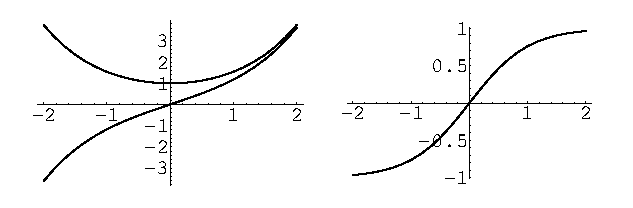
\includegraphics[height=1.5in]{appendix/sicotanh}
  \end{center}
  \caption{Hyperbolic cosine, sine and tangent.}
  \label{sicotanh}
\end{figure}









\raggedbottom
%%===========================================================================
\chapter{Bessel Functions}
\flushbottom

%%CONTINUE HERE

\section{Definite Integrals}

Let $\nu > -1$.
\begin{gather*}
  \int_0^1 r J_\nu(j_{\nu,m} r) J_\nu(j_{\nu,n} r) \,\dd r 
  = \frac{1}{2} \left( {J'}_\nu(j_{\nu,n}) \right)^2 \delta_{m n} 
  \\
  \int_0^1 r J_\nu({j'}_{\nu,m} r) J_\nu({j'}_{\nu,n} r) \,\dd r 
  = \frac{{j'}_{\nu,n}^2 - \nu^2}{2 {j'}_{\nu,n}^2} 
  \left( J_\nu({j'}_{\nu,n}) \right)^2 \delta_{m n} 
  \\
  \int_0^1 r J_\nu(\alpha_m r) J_\nu(\alpha_n r) \,\dd r 
  = \frac{1}{2 \alpha_n^2} \left( \frac{a^2}{b^2}
    + \alpha_n^2 - \nu^2 \right)
  \left( J_\nu(\alpha_n) \right)^2 \delta_{m n}
\end{gather*}
Here $\alpha_n$ is the $n^{\mathrm{th}}$ positive root of 
$a J_\nu(r) + b r {J'}_\nu(r)$, where $a,b \in \mathbb{R}$.







\raggedbottom
%%===========================================================================
\chapter{Formulas from Linear Algebra}
\label{appendix formulas from linear algebra}
\flushbottom

\paragraph{Kramer's Rule.}
\index{Kramer's rule}

Consider the matrix equation
\[ A \vec{x} = \vec{b}. \]
This equation has a unique solution if and only if $\det(A) \neq 0$.  
If the determinant vanishes then there are either no solutions or an 
infinite number of solutions.
If the determinant is nonzero, the solution for each $x_j$ can be written
\[ x_j = \frac{\det A_j}{\det A} \]
where $A_j$ is the matrix formed by replacing the $j^{t h}$ column of $A$ 
with $b$.

\begin{Example}
  The matrix equation
  \[ \begin{pmatrix}
    1       &       2 \\
    3       &       4 
  \end{pmatrix}
  \begin{pmatrix}
    x_1 \\
    x_2
  \end{pmatrix}
  = 
  \begin{pmatrix}
    5 \\
    6
  \end{pmatrix},
  \]
  has the solution
  \[ x_1 = \frac{
    \begin{vmatrix}
      5       &       2 \\
      6       &       4
    \end{vmatrix} }{
    \begin{vmatrix}
      1       &       2 \\
      3       &       4
    \end{vmatrix} }
  = \frac{8}{-2} = -4, \qquad
  x_2 = \frac{
    \begin{vmatrix}
      1       &       5 \\
      3       &       6
    \end{vmatrix} }{
    \begin{vmatrix}
      1       &       2 \\
      3       &       4
    \end{vmatrix} }
  = \frac{-9}{-2} = \frac{9}{2}.
  \]
\end{Example}













\raggedbottom
%%=============================================================================
\chapter{Vector Analysis}
\flushbottom

\paragraph{Rectangular Coordinates}

\[
f = f(x,y,z), \qquad \vec{g} = g_x \mathbf{i} + g_y \mathbf{j} + g_z \mathbf{k}
\]

\[
\nabla f = \frac{\partial f}{\partial x} \mathbf{i} + \frac{\partial f}{\partial y} \mathbf{j} + \frac{\partial f}{\partial z} \mathbf{k}
\]

\[
\nabla \cdot \vec{g} = \frac{\partial g_x}{\partial x} + \frac{\partial g_y}{\partial y}
+ \frac{\partial g_z}{\partial z}
\]

\[
\nabla \times \vec{g} =
\begin{vmatrix}
  \mathbf{i} & \mathbf{j} & \mathbf{k} \\
  \frac{\partial}{\partial x} & \frac{\partial}{\partial y} & \frac{\partial}{\partial z} \\
  g_x & g_y & g_z
\end{vmatrix}
\]

\[
\Delta f = \nabla^2 f = \frac{\partial^2 f}{\partial x^2} + \frac{\partial^2 f}{\partial y^2} + \frac{\partial^2 f}{\partial z^2}
\]


\paragraph{Spherical Coordinates}

\[
x = r \cos \theta \sin \phi, \qquad
y = r \sin \theta \sin \phi, \qquad
z = r \cos \phi
\]

\[
f = f(r, \theta, \phi), \qquad \vec{g} = 
g_r \mathbf{r} + g_\theta \boldsymbol{\theta} + g_\phi \boldsymbol{\phi}
\]


%%CONTINUE

%%\paragraph{Cylindrical Coordinates}


%%CONTINUE



\paragraph{Divergence Theorem.}
\[
\iint \nabla \cdot \mathbf{u} \,\dd x \,\dd y 
= \oint \mathbf{u} \cdot \mathbf{n} \,\dd s
\]

\paragraph{Stoke's Theorem.}
\[
\iint (\nabla \times \mathbf{u}) \cdot \,\dd \mathbf{s}
= \oint \mathbf{u} \cdot \,\dd \mathbf{r}
\]

%% CONTINUE








\raggedbottom
%%=============================================================================
\chapter{Partial Fractions}
\flushbottom



%%CONTINUE: Check this.


A proper rational function
\[
\frac{p(x)}{q(x)} = \frac{p(x)}{(x-a)^n r(x)}
\]
Can be written in the form
\[
\frac{p(x)}{(x-\alpha)^n r(x)} = \left( \frac{a_0}{(x-\alpha)^n} 
  + \frac{a_1}{(x-\alpha)^{n-1}} + \cdots + \frac{a_{n-1}}{x-\alpha}
\right) + (\cdots)
\]
where the $a_k$'s are constants and the last ellipses represents the 
partial fractions expansion of the roots of $r(x)$.  The coefficients are
\[
a_k = \frac{1}{k!} \frac{d^k}{d x^k} 
\left( \frac{p(x)}{r(x)} \right) \bigg|_{x=\alpha}.
\]



\begin{Example}
  Consider the partial fraction expansion of 
  \[
  \frac{1+x+x^2}{(x-1)^3}.
  \]
  The expansion has the form
  \[
  \frac{a_0}{(x-1)^3} + \frac{a_1}{(x-1)^2} + \frac{a_2}{x-1}.
  \]
  The coefficients are
  \begin{align*}
    a_0     &= \frac{1}{0!} (1+x+x^2)|_{x=1} = 3, \\
    a_1     &= \frac{1}{1!} \frac{\dd}{\dd x}(1+x+x^2)|_{x=1} 
    = (1+2x)|_{x=1} = 3, \\
    a_2     &= \frac{1}{2!} \frac{\dd^2}{\dd x^2}(1+x+x^2)|_{x=1} 
    = \frac{1}{2} (2)|_{x=1} = 1.
  \end{align*}
  Thus we have
  \[
  \frac{1+x+x^2}{(x-1)^3} = \frac{3}{(x-1)^3} + \frac{3}{(x-1)^2} 
  + \frac{1}{x-1}.
  \]
\end{Example}



\begin{Example}
  Consider the partial fraction expansion of 
  \[
  \frac{1+x+x^2}{x^2 (x-1)^2}.
  \]
  The expansion has the form
  \[
  \frac{a_0}{x^2} + \frac{a_1}{x} + \frac{b_0}{(x-1)^2} + \frac{b_1}{x-1}.
  \]
  The coefficients are
  \begin{align*}
    a_0     &= \frac{1}{0!} \left( \frac{1+x+x^2}{(x-1)^2} \right)
    \bigg|_{x=0} = 1, \\
    a_1     &= \frac{1}{1!} \frac{\dd}{\dd x} 
    \left( \frac{1+x+x^2}{(x-1)^2} \right) \bigg|_{x=0} 
    = \left( \frac{1+2x}{(x-1)^2} 
      - \frac{2(1+x+x^2)}{(x-1)^3} \right) \bigg|_{x=0}
    = 3, \\
    b_0     &= \frac{1}{0!} \left( \frac{1+x+x^2}{x^2} \right)
    \bigg|_{x=1} = 3, \\
    b_1     &= \frac{1}{1!} \frac{\dd}{\dd x} 
    \left( \frac{1+x+x^2}{x^2} \right) \bigg|_{x=1} 
    = \left( \frac{1+2x}{x^2} 
      - \frac{2(1+x+x^2)}{x^3} \right) \bigg|_{x=1}
    = -3, 
  \end{align*}
  Thus we have
  \[
  \frac{1+x+x^2}{x^2 (x-1)^2} = \frac{1}{x^2} + \frac{3}{x} 
  + \frac{3}{(x-1)^2} - \frac{3}{x-1}.
  \]
\end{Example}





If the rational function has real coefficients and the denominator 
has complex roots, then you can reduce the work in finding the partial 
fraction expansion with the following trick:  Let $\alpha$ and $\overline{\alpha}$
be complex conjugate pairs of roots of the denominator.
\begin{align*}
  \frac{p(x)}{(x-\alpha)^n (x- \overline{\alpha})^n r(x)} 
  &= \left( \frac{a_0}{(x-\alpha)^n} 
    + \frac{a_1}{(x-\alpha)^{n-1}} + \cdots + \frac{a_{n-1}}{x-\alpha}
  \right) \\
  &\quad + \left( \frac{\overline{a_0}}{(x-\overline{\alpha})^n} 
    + \frac{\overline{a_1}}{(x-\overline{\alpha})^{n-1}} + \cdots 
    + \frac{\overline{a_{n-1}}}{x-\overline{\alpha}} \right) 
  + (\cdots)
\end{align*}
Thus we don't have to calculate the coefficients for the root at 
$\overline{\alpha}$.  We just take the complex conjugate of the coefficients
for $\alpha$.





\begin{Example}
  Consider the partial fraction expansion of 
  \[
  \frac{1+x}{x^2+1}.
  \]
  The expansion has the form
  \[
  \frac{a_0}{x-i} + \frac{\overline{a_0}}{x+i} 
  \]
  The coefficients are
  \begin{align*}
    a_0     &= \frac{1}{0!} \left(\frac{1+x}{x+i} \right) 
    \bigg|_{x=i} = \frac{1}{2}(1-i), \\
    \overline{a_0} &= \overline{ \frac{1}{2}(1-i)} = \frac{1}{2}(1+i)
  \end{align*}
  Thus we have
  \[
  \frac{1+x}{x^2+1} = \frac{1-i}{2(x-i)} + \frac{1+i}{2(x+i)}.
  \]
\end{Example}












\raggedbottom
%%=============================================================================
\chapter{Finite Math}
\flushbottom


\paragraph{Newton's Binomial Formula.}
\index{Newton's binomial formula}
\index{binomial formula}
\begin{align*}
  (a+b)^n &= \sum_{k=0}^n \binom{k}{n} a^{n-k} b^k \\
  &= a^n + n a^{n-1} b + \frac{n(n-1)}{2} a^{n-2} b^2 + \cdots 
  + n a b^{n-1} + b^n,
\end{align*}
The \textit{binomial coefficients} are,
\index{binomial coefficients}
\[
\binom{k}{n} = \frac{n!}{k! (n-k)!}.
\]


\raggedbottom
%%=============================================================================
\chapter{Physics}
\label{chapter spherical chicken}
\index{spherical chicken}
\index{chicken!spherical}
\flushbottom


In order to reduce processing costs, a chicken farmer wished to acquire
a plucking machine.  Since there was no such machine on the market, 
he hired a mechanical engineer to design one.  After extensive
research and testing, the professor concluded that it was impossible to 
build such a machine with current technology.  The farmer was disappointed,
but not wanting to abandon his dream of an automatic plucker, he consulted
a physicist.  After a single afternoon of work, the physicist reported 
that not only could a plucking machine be built, but that the design 
was simple.  The elated farmer asked him to describe his method.
The physicist replied, ``First, assume a spherical chicken \ldots''.

The problems in this text will implicitly make certain simplifying 
assumptions about chickens.  For example, a problem might assume 
a perfectly elastic, frictionless, spherical chicken.  In two-dimensional
problems, we will assume that chickens are circular.





\raggedbottom
%%=============================================================================
\chapter{Probability}
\flushbottom




\section{Independent Events}

Once upon a time I was talking with the father of one of my colleagues
at Caltech.  He was an educated man.  I think that he had studied
Russian literature and language back when he was in college.  We were
discussing gambling.  He told me that he had a scheme for winning money
at the game of 21.  I was familiar with counting cards.  Being a mathematician,
I was not interested in hearing about conditional probability from a 
literature major, but I said nothing and prepared to hear about his particular 
technique.  I was quite surprised with his ``method'':  He said that when he 
was on a winning streak he would bet more and when he was on a losing streak
he would bet less.  He conceded that he lost more hands than he won, 
but since he bet more when he was winning, he made money in the end.  

I respectfully and thoroughly explained to him the concept of an independent
event.  Also, if one is not counting cards then each hand
in 21 is essentially an independent event.  The outcome of the previous
hand has no bearing on the current.  Throughout the explanation he nodded
his head and agreed with my reasoning.  When I was finished he replied,
``Yes, that's true.  But you see, I have a method.  When I'm on my winning
streak I bet more and when I'm on my losing streak I bet less.''  

I pretended
that I understood.  I didn't want to be rude.  After all, he had taken the 
time to explain the concept of a winning streak to me.  And everyone knows
that mathematicians often do not easily understand practical matters, 
particularly games of chance.

\textit{
  Never explain mathematics to the layperson.  
  }



\section{Playing the Odds}


Years ago in a classroom not so far away, your author was being subjected
to a presentation of a lengthy proof.   About five minutes into the 
lecture, the entire class was hopelessly lost.  At the forty-five minute
mark the professor had a combinatorial expression that covered most of
a chalk board.  From his previous queries the professor knew that none
of the students had a clue what was going on.  This pleased him and 
he had became more animated as the lecture had progressed.  He gestured
to the board with a smirk and asked for the value of the expression.
Without a moment's hesitation, I nonchalantly replied, ``zero''.  
The professor was taken aback.  He was clearly impressed that I was able
to evaluate the expression, especially because I had done it in my head
and so quickly.  He enquired as to my method.
``Probability'', I replied.  ``Professors often present difficult problems
that have simple, elegant solutions.  Zero is the most elegant of 
numerical answers and thus most likely to be the correct answer.  My second
guess would have been one.''  The professor was not amused.




Whenever a professor asks the class a question which has a numeric answer,
immediately respond, ``zero''.  If you are asked about your method, casually
say something vague about symmetry.  Speak with confidence and give 
non-verbal cues that you consider the problem to be elementary.
This tactic will usually suffice.  It's quite likely that some kind of 
symmetry is involved.  And if it isn't your response will puzzle the professor.
They may continue with the next topic, not wanting to admit that they
don't see the ``symmetry'' in such an elementary problem.  If they press
further, start mumbling to yourself.  Pretend that you are lost in thought,
perhaps considering some generalization of the result.   They may be a 
little irked that you are ignoring them, but it's better than divulging
your true method.













\raggedbottom
%%=============================================================================
\chapter{Economics}
\flushbottom


\index{economics}
\index{opportunity cost}
\index{computer games}
\paragraph{}
There are two important concepts in economics.  The first is ``Buy
low, sell high'', which is self-explanitory.  The second is
\textit{opportunity cost}, the highest valued alternative that must be
sacrificed to attain something or otherwise satisfy a want.  I
discovered this concept as an undergraduate at Caltech.  I was never
very interested in computer games, but one day I found myself randomly
playing tetris.  Out of the blue I was struck by a revelation: ``I
could be having sex right now.''  I haven't played a computer game
since.




\raggedbottom
%%=============================================================================
\chapter{Glossary}
\flushbottom


\paragraph{}
Phrases often have different meanings in mathematics than in everyday usage.
Here I have collected definitions of some mathematical terms which might
confuse the novice.


\begin{description}
\item{\textbf{beyond the scope of this text:}}
  Beyond the comprehension of the author.
\item{\textbf{difficult:}}
  Essentially impossible.  Note that mathematicians never refer to problems 
  they have solved as being difficult.  This would either be boastful, 
  (claiming that you can solve difficult problems), or self-deprecating,
  (admitting that you found the problem to be difficult).
\item{\textbf{interesting:}}
  This word is grossly overused in math and science.
  It is often used to describe any work that the author has done, regardless 
  of the work's significance or novelty.
  It may also be used as a synonym for difficult.
  It has a completely different meaning when used by the non-mathematician.
  When I tell people that I am a mathematician they typically respond 
  with, ``That must be interesting.'', which means, ``I don't know 
  anything about math or what mathematicians do.''  I typically answer,
  ``No.  Not really.''  
\item{\textbf{non-obvious} or \textbf{non-trivial:}}
  Real fuckin' hard.
\item{\textbf{one can prove that \ldots:}}
  The ``one'' that proved it was a genius like Gauss.  The phrase literally 
  means ``you haven't got a chance in hell of proving that \ldots''
\item{\textbf{simple:}}
  Mathematicians communicate their prowess to colleagues and students by 
  referring to all problems as simple or trivial.  If you ever become a math
  professor, introduce every example as being ``really quite trivial.''
  \footnote{For even more fun say it in your best Elmer Fudd accent.
    ``This next pwobwem is weawy quite twiviaw''.}
\end{description}



\paragraph{}
Here are some less interesting words and phrases that you are 
probably already familiar with.

\begin{description}
\item{\textbf{corollary:}}
  a proposition inferred immediately from a proved proposition with little 
  or no additional proof
\item{\textbf{lemma:}}
  an auxiliary proposition used in the demonstration of another proposition
\item{\textbf{theorem:}}
  a formula, proposition, or statement in mathematics or logic deduced or 
  to be deduced from other formulas or propositions
\end{description}


\raggedbottom
%%=============================================================================
\chapter{whoami}
\flushbottom

\begin{figure}[h!]
  \begin{center}
    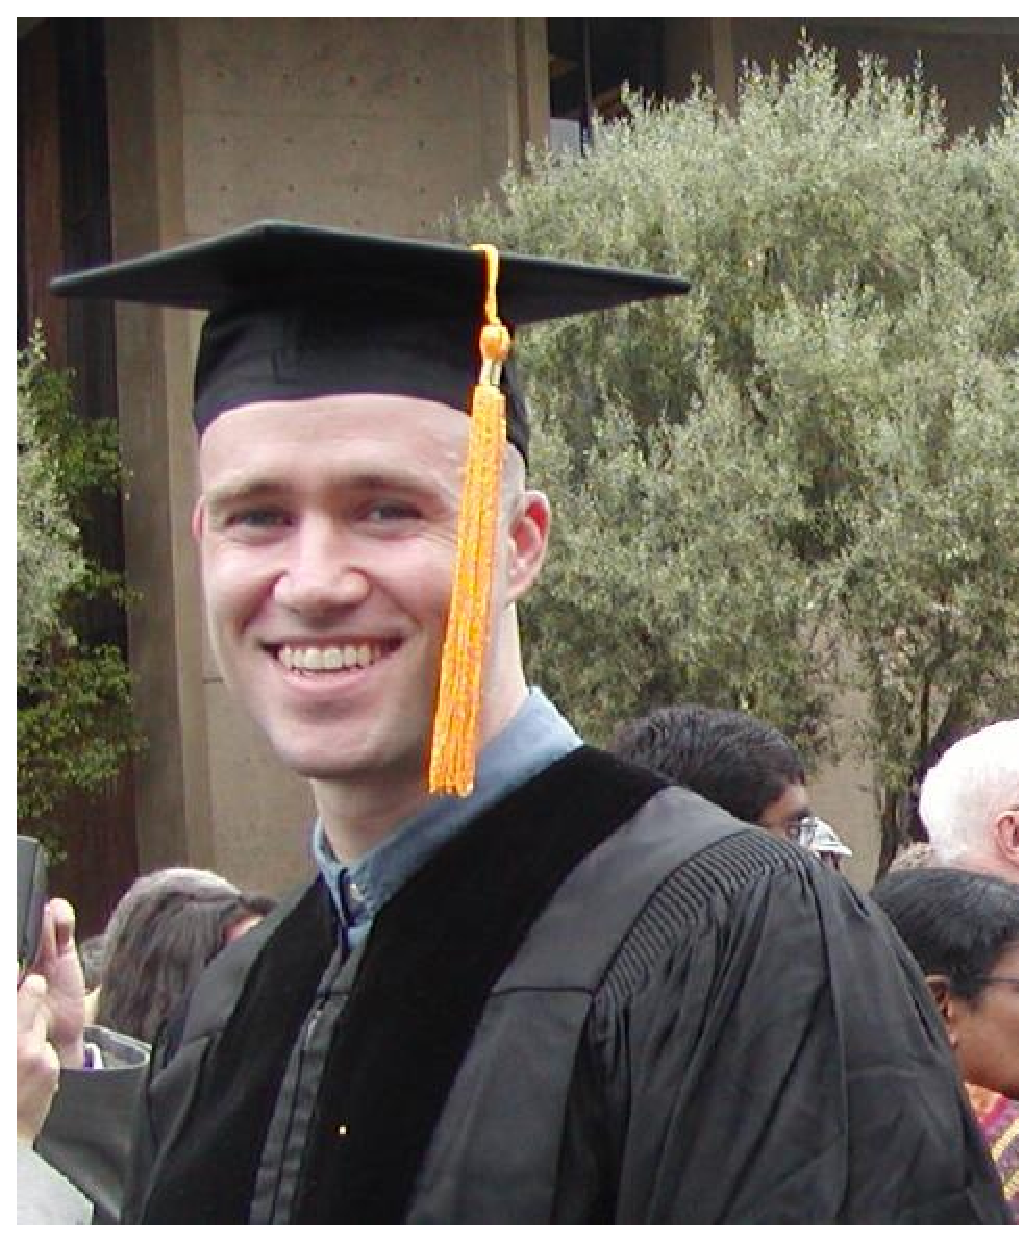
\includegraphics[width=0.5\textwidth]{appendix/graduation}
  \end{center}
  \caption{Graduation, June 13, 2003.}
  \label{figure graduation}
\end{figure}

\raggedbottom
